\documentclass[12pt]{ociamthesis}  % default square logo 
%\documentclass[12pt,beltcrest]{ociamthesis} % use old belt crest logo
%\documentclass[12pt,shieldcrest]{ociamthesis} % use older shield crest logo

%load any additional packages
\usepackage{amssymb}
\usepackage{listings}
\usepackage{color}

\definecolor{codegreen}{rgb}{0,0.6,0}
\definecolor{codegray}{rgb}{0.5,0.5,0.5}
\definecolor{codepurple}{rgb}{0.58,0,0.82}
\definecolor{backcolour}{rgb}{0.95,0.95,0.92}

\lstdefinestyle{mystyle}{
    backgroundcolor=\color{backcolour},   
    commentstyle=\color{codegreen},
    keywordstyle=\color{magenta},
    numberstyle=\tiny\color{codegray},
    stringstyle=\color{codepurple},
    basicstyle=\footnotesize,
    breakatwhitespace=false,         
    breaklines=true,                 
    captionpos=b,                    
    keepspaces=true,                 
    numbers=left,                    
    numbersep=5pt,                  
    showspaces=false,                
    showstringspaces=false,
    showtabs=false,                  
    tabsize=2,
    language=sh
}

\lstset{style=mystyle}

%input macros (i.e. write your own macros file called mymacros.tex 
%and uncomment the next line)
%\include{mymacros}

\title{Modul Praktikum \\[1ex]     %your thesis title,
        Kecerdasan Buatan}   %note \\[1ex] is a line break in the title

\author{Rolly Maulana Awangga}             %your name
\college{0410118609\\[5ex]
Applied Bachelor of Informatics Engineering}  %your college

%\renewcommand{\submittedtext}{change the default text here if needed}
\degree{Politeknik Pos Indonesia}     %the degree
\degreedate{Bandung 2019}         %the degree date

%end the preamble and start the document
\begin{document}

%this baselineskip gives sufficient line spacing for an examiner to easily
%markup the thesis with comments
\baselineskip=18pt plus1pt

%set the number of sectioning levels that get number and appear in the contents
\setcounter{secnumdepth}{3}
\setcounter{tocdepth}{3}


\maketitle                  % create a title page from the preamble info
\include{section/dedication}        % include a dedication.tex file
\include{section/acknowlegements}   % include an acknowledgements.tex file
\include{section/abstract}          % include the abstract

\begin{romanpages}          % start roman page numbering
\tableofcontents            % generate and include a table of contents
\listoffigures              % generate and include a list of figures
\end{romanpages}            % end roman page numbering

%now include the files of latex for each of the chapters etc
\chapter{Mengenal Kecerdasan Buatan dan Scikit-Learn}
Buku umum yang digunakan adalah \cite{russell2016artificial} dan  
untuk sebelum UTS menggunakan buku \textit{Python Artificial Intelligence Projects for Beginners}\cite{eckroth2018python}.
Dengan praktek menggunakan python 3 dan editor anaconda dan library python scikit-learn.
Tujuan pembelajaran pada pertemuan pertama antara lain:
\begin{enumerate}
\item
Mengerti definisi kecerdasan buatan, sejarah kecerdasan buatan, perkembangan dan penggunaan di perusahaan
\item
Memahami cara instalasi dan pemakaian sci-kit learn
\item
Memahami cara penggunaan variabel explorer di spyder
\end{enumerate}
Tugas dengan cara dikumpulkan dengan pull request ke github dengan menggunakan latex pada repo yang dibuat oleh asisten riset.

\section{Teori}
Praktek teori penunjang yang dikerjakan :
\begin{enumerate}
\item
Buat Resume Definisi, Sejarah dan perkembangan Kecerdasan Buatan, dengan bahasa yang mudah dipahami dan dimengerti. Buatan sendiri bebas plagiat[hari ke 1](10)
\item
Buat Resume mengenai definisi supervised learning, klasifikasi, regresi dan unsupervised learning. Data set, training set dan testing set.[hari ke 1](10)
\end{enumerate}

\section{Instalasi}
Membuka https://scikit-learn.org/stable/tutorial/basic/tutorial.html. Dengan menggunakan bahasa yang mudah dimengerti dan bebas plagiat. 
Dan wajib skrinsut dari komputer sendiri.
\begin{enumerate}
\item
Instalasi library scikit dari anaconda, mencoba kompilasi dan uji coba ambil contoh kode dan lihat variabel explorer[hari ke 1](10)
\item
Mencoba Loading an example dataset, menjelaskan maksud dari tulisan tersebut dan mengartikan per baris[hari ke 1](10)
\item
Mencoba Learning and predicting, menjelaskan maksud dari tulisan tersebut dan mengartikan per baris[hari ke 2](10)
\item
mencoba Model persistence, menjelaskan maksud dari tulisan tersebut dan mengartikan per baris[hari ke 2](10)
\item 
Mencoba Conventions, menjelaskan maksud dari tulisan tersebut dan mengartikan per baris[hari ke 2](10)
\end{enumerate}


\section{Penanganan Error}
Dari percobaan yang dilakukan di atas, apabila mendapatkan error maka:

\begin{enumerate}
	\item
	skrinsut error[hari ke 2](10)
	\item
Tuliskan kode eror dan jenis errornya [hari ke 2](10)
	\item
Solusi pemecahan masalah error tersebut[hari ke 2](10)

\end{enumerate}

<<<<<<< HEAD
\section{Teori/Mhd Zulfikar Akram Nasution/1164081}
\begin{enumerate}
\item Definisi, Sejarah dan Perkembangan Kecerdasan Buatan
\begin{itemize}
\item Definisi
\par
Kecerdasan Buatan adalah kecerdasan yang ditambahkan kepada suatu sistem yang bisa diatur dalam konteks ilmiah yang berhubungan dengan pemanfaatan mesin untuk memecahkan persoalan yang rumit dengan cara yang lebih manusiawi. 
\par
\item Sejarah dan Perkembangan
\par
Sejarah dan perkembangan kecerdasan buatan terjadi pada musim panas tahun 1956 tercatat adanya seminar mengenai AI di Darmouth College. Seminar pada waktu itu dihadiri oleh sejumlah pakar komputer dan membahas potensi komputer dalam meniru kepandaian manusia. Akan tetapi perkembangan yang sering terjadi semenjak diciptakannya LISP, yaitu bahasa kecerdasan buatan yang dibuat tahun 1960 oleh John McCarthy. Istilah pada kecerdasan buatan atau Artificial Intelligence diambil dari Marvin Minsky dari MIT. Dia menulis karya ilmiah berjudul Step towards Artificial Intelligence,The Institute of radio Engineers Proceedings 49, January 1961.
\end{itemize}

\item Definisi Supervised Learning, Unsupervised Learning, Klasifikasi, Regresi, Data Set, Training Set dan Testing Set
\begin{itemize}
\item Supervised Learning dan Unsupervised Learning
\par
Supervised learning merupakan sebuah pendekatan dimana sudah terdapat data yang dilatih, dan terdapat variable yang ditargetkan sehingga tujuan dari pendekatan ini adalah mengkelompokan suatu data ke data yang sudah ada. Sedangkan unsupervised learning tidak memiliki data latih, sehingga dari data yang ada, kita mengelompokan data tersebut menjadi 2 bagian atau 3 bagian dan seterusnya.
\item Klasifikasi
\par
Klasifikasi adalah salah satu topik utama dalam data mining atau machine learning. Klasifikasi yaitu suatu pengelompokan data dimana data yang digunakan tersebut mempunyai kelas label atau target.
\item Regresi
\par
Regresi adalah Supervised learning tidak hanya mempelajari classifier, tetapi juga mempelajari fungsi yang dapat memprediksi suatu nilai numerik. Contoh, ketika diberi foto seseorang, kita ingin memprediksi umur, tinggi, dan berat orang yang ada pada foto tersebut.
\item Data Set
\par
Data set adalah cabang aplikasi dari Artificial Intelligence/Kecerdasan Buatan yang fokus pada pengembangan sebuah sistem yang mampu belajar sendiri tanpa harus berulang kali di program oleh manusia.
\item Training Set
\par
Training set yaitu jika pasangan objek, dan kelas yang menunjuk pada objek tersebut adalah suatu contoh yang telah diberi label akan menghasilkan suatu algoritma pembelajaran.
\item Testing Set
\par
Testing set digunakan untuk mengukur sejauh mana classifier berhasil melakukan klasifikasi dengan benar.
\end{itemize}
\item Instalasi Scikit-Learn dari Anaconda
\begin{itemize}
\item Pertama install Anaconda di pc masing-masing
\item Kemudian buka cmd untuk menginstall scikit-learn
\item Ketik perintah "conda install scikit-learn" dan pilih "y"
\end{itemize}
\begin{figure}[ht]
\centering
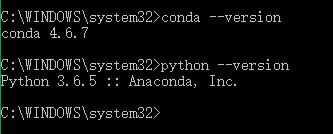
\includegraphics[scale=0.6]{figures/1.png}
\caption{Install Scikit-Learn Conda}
\label{Proses Instalasi}
\end{figure}
\begin{itemize}
\item Lalu ketik "pip install -U scikit-learn" untuk memasukkan anaconda ke python
\end{itemize}
\begin{figure}[ht]
\centering
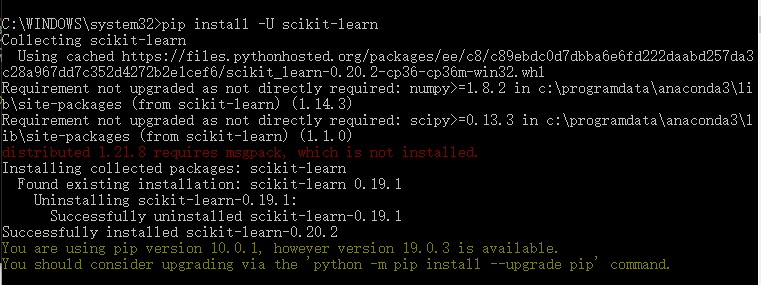
\includegraphics[scale=0.5]{figures/2.png}
\caption{Install Scikit-Learn ke Python}
\label{Gabung Conda dan Python}
\end{figure}
\begin{itemize}
\item Setelah itu, kompilasi kode di dalam python dengan ketik "python", lalu "print('Zulfikar')" maka akan menghasilkan seperti gambar berikut.
\end{itemize}
\begin{figure}[ht]
\centering
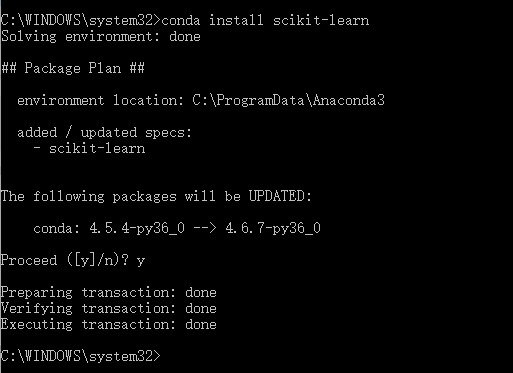
\includegraphics[scale=0.6 ]{figures/3.png}
\caption{Kompilasi Kode}
\label{Kompilasi Kode}
\end{figure}
\item Loading an Example Dataset
\begin{itemize}
\item Ketik perintah berikut "from sklearn import datasets" untuk mengimport dataset dari sklearn.
\end{itemize}
\begin{figure}[ht]
\centering
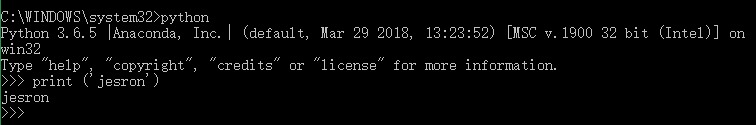
\includegraphics[scale=0.5]{figures/4.png}
\caption{Import Datasets}
\label{Import Datasets}
\end{figure}
\begin{itemize}
\item Kemudian ketik perintah berikut  untuk membuat variable iris yang berisi datasets.
\end{itemize}
\begin{figure}[ht]
\centering

\includegraphics[scale=0.9]{figures/5.png}
\caption{Buat variable iris}
\label{Variable Iris}
\end{figure}
\begin{itemize}
\item Lalu ketik perintah berikut untuk membuat variable digits yang berisi datasets, dan juga untuk melihat isi data dari datasets seperti gambar 1.6 .
\end{itemize}
\begin{figure}[ht]
\centering
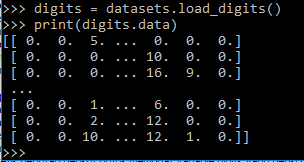
\includegraphics[scale=0.7]{figures/8.png}
\caption{Buat variable digits}
\label{Variable Digits}
\end{figure}
\end{enumerate}

\section{Jesron Marudut Hatuan/1164077}
\subsection{Teori}
\begin{enumerate}
\item Definisi, sejarah, dan perkembangan kecerdasan buatan.
\subitem Kecerdasan Buatan (Artificial Intelligence atau AI) dapat didefinisikan sebagai kecerdasan yang ditunjukkan oleh suatu entitas buatan. Sistem seperti ini biasanya dianggap komputer. Kecerdasan diciptakan lalu dimasukkan ke dalam suatu mesin atau komputer supaya dapat melakukan pekerjaan-pekerjan yang dapat dilakukan manusia.
\subitem Sebenarnya area Kecerdasan Buatan (Artificial Intelligence) atau disingkat dengan AI, dimulai dari munculanya komputer sekitar tahun 1940-an, meskipun sejarah perkembangannya dapat dilacak dari zaman Mesir kuno. Pada akhir tahun 1955, Newell dan Simon mengembangkan The Logic Theorist atau program AI terdahulu. Program ini merepresentasikan masalah sebagai model pohon, lalu penyelesaiannya dengan  memilih cabang yang akan menghasilkan kesimpulan terbenar. Program tersebut berdampak besar dan menjadi batu loncatan dalam mengembangkan bidang AI. Pada tahun 1956 John McCarthy dari  Massacuhetts Institute of Technology dianggap sebagai bapak AI, menyelenggarakan konferensi untuk menarik para ahli komputer bertemu, dengan  nama kegiatan The Dartmouth Summer Research Project On AI. Konferensi Dartmouth saat itu mempertemukan para pendiri dalam AI, dan bertugas untuk meletakkan dasar bagi masa depan  pemgembangan dan penelitian AI. John McCarthy  disaat itu mengusulkan definisi AI adalah AI merupakan cabang dari ilmu komputer yang berfokus pada pengembangan komputer agar mempunyai kemampuan dan berprilaku seperti manusia.
\item  Definisi supervised learning, klasifikasi, regresi, dan unsupervised learning. Data set, training set dan testing set. 
\subitem Supervised learning merupakan sebuah pendekatan dimana sudah terdapat data yang dilatih, dan terdapat variable yang ditargetkan sehingga tujuan dari pendekatan ini adalah mengkelompokan suatu data ke data yang sudah ada. Sedangkan unsupervised learning tidak memiliki data latih, sehingga dari data yang ada, kita mengelompokan data tersebut menjadi 2 bagian atau 3 bagian dan seterusnya.
\subitem Klasifikasi adalah salah satu topik utama dalam data mining atau machine learning. Klasifikasi yaitu suatu pengelompokan data dimana data yang digunakan tersebut mempunyai kelas label atau target.
\subitem Regresi adalah Supervised learning tidak hanya mempelajari classifier, tetapi juga mempelajari fungsi yang dapat memprediksi suatu nilai numerik. Contoh, ketika diberi foto seseorang, kita ingin memprediksi umur, tinggi, dan berat orang yang ada pada foto tersebut.
\subitem Data set adalah cabang aplikasi dari Artificial Intelligence/Kecerdasan Buatan yang fokus pada pengembangan sebuah sistem yang mampu belajar sendiri tanpa harus berulang kali di program oleh manusia.
\subitem Training set yaitu jika pasangan objek, dan kelas yang menunjuk pada objek tersebut adalah suatu contoh yang telah diberi label akan menghasilkan suatu algoritma pembelajaran.
\subitem Testing set digunakan untuk mengukur sejauh mana classifier berhasil melakukan klasifikasi dengan benar\cite{zhu2009introduction}.
\end{enumerate}


\subsection{Instalasi}
\subsubsection{Instalasi Library Scikit dari Anaconda}
\begin{enumerate}
\item Sediakan aplikasi Anaconda terlebih dahulu
\begin{figure}[ht]
\centerline{
\includegraphics[width=1\textwidth]{figures/0.PNG}}
\caption{Applikasi Anaconda.}
\end{figure}
\item Setelah di install, masukkan script dibawah ini untuk melihat versi Python dan Anacondanya
\begin{figure}[ht]
\centerline{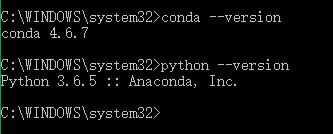
\includegraphics[width=0.75\textwidth]{figures/1.JPEG}}
\caption{Versi Anaconda.}
\end{figure}
\item  Selanjutnya masukkan perintah 'pip install -U scikit-learn'
\begin{figure}[ht]
\centerline{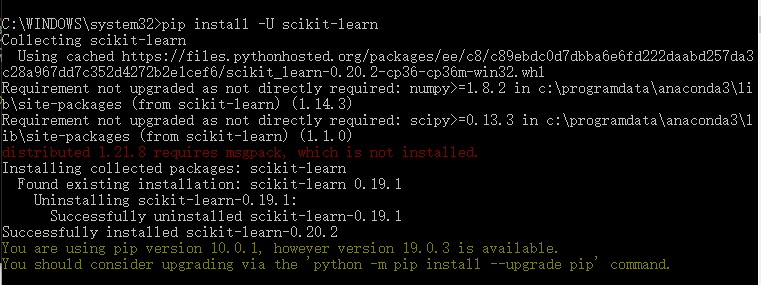
\includegraphics[width=0.75\textwidth]{figures/2.JPEG}}
\caption{Instalasi.}
\end{figure}
\item  Selanjutnya masukkan perintah 'conda install  scikit-learn'
\begin{figure}[ht]
\centerline{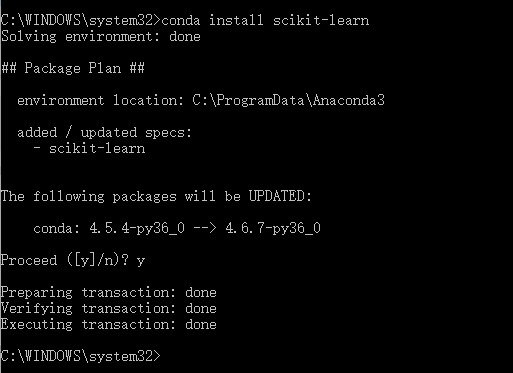
\includegraphics[width=0.75\textwidth]{figures/3.JPEG}}
\caption{Langkah installasi anaconda.}
\end{figure}
\item  Selanjutnya masukkan perintah 'python' dan 'print ('jesron')
\begin{figure}[ht]
\centerline{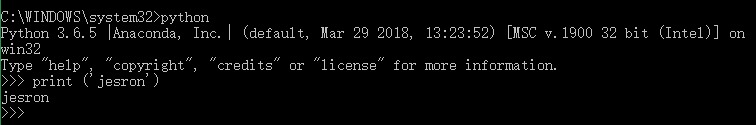
\includegraphics[width=0.5\textwidth]{figures/4.JPEG}}
\caption{Langkah terakhir.}
\end{figure}
\end{enumerate}

<<<<<<< HEAD


=======
\section{Teori/Puad Hamdani/1164084}
\begin{enumerate}
\item Definisi, Sejarah dan Perkembangan Kecerdasan Buatan
\begin{itemize}
\item Definisi
\par
Kecerdasan buatan adalah ilmu pengetahuan yang berhubungan dengan mesin untuk memecahkan persoalan rumit dengan cara yang mudah,dilakukan dengan mengikuti kecerdasan manusia dan menerapkanya di computer sebagai algoritma
\par
\item Sejarah dan Perkembangan
\par
AI (artificial Intelligence) di kenal sekitar tahun 1943 Teori tentang jaringan saraf tiruan (artificial neuron network, ANN) menyatakan bahwa setiap neuron dapat dimisalkan dalam keadaan biner, yaitu ON dan OFF. Dari setiap percobaan, setiap fungsi perhitungan dapat diselesaikan melalui jaringan neuron yang dimodelkan.
Pada tahun 1965, Lotfi Zadeh, professor teknik elektro di University of California, memublikasikan konsepnya yang disebut dengan “fuzzy sets”. Beliau menjabarkan FL dengan pernyataan matematis dan visual yang mudah dipahami. Karena kajian ini berkaitan dengan sistem kontrol, konsep tersebut banyak dikembangkan dalam konteks pemrograman komputer hingga saat ini.
\end{itemize}
\item Definisi Supervised Learning, Unsupervised Learning, Klasifikasi, Regresi, Data Set, Training Set dan Testing Set
\begin{itemize}
\item Supervised Learning 
\par
Supervised learning adalah pembelajaran yang terawasi dimana jika output yang diharapkan telah diketahui sebelumnya. Biasanya pembelajaran ini dilakukan dengan menggunakan data yang telah ada
\item Unsupervised Learning
\par
Unsupervised learning adalah pembelajaran yang tidak terawasi dimana tidak memerlukan target output. Metode ini tidak dapat ditentukan hasil seperti apa yang diharapkan selama proses pembelajaran, Nilai bobot yang disusun dalam proses range tertentu tergantung pada output yang diberikan.
\item Klasifikasi
\par
Klasifikasi adalah Proses pengelompokkan berdasarkan ciri-ciri persamaan dan perbedaan
\item Regresi
\par
Regresi adalah metode analisis statistik yang digunakan untuk melihat pengaruh antara dua atau lebih variabel
\item Data Set
\par
Data set adalah objek yang merepresentasikan data dan relasinya di memory, Strukturnya hampir mirip dengan data di data base. Data set berisi koleksi dari data table dan data relation 
\item Training Set
\par
Training set adalah bagian dataset yang kita latih untuk membuat prediksi atau algoritma ML lainnya sesuai tujuannya masing-masing. Kita memberikan petunjuk melalui algoritma agar mesin yang kita latih bisa mencari korelasinya sendiri. Walau demikian proses belajar harusnya proporsional. Layaknya seorang murid yang terlalu diforsir belajar, maka hasilnya pun tidak akan baik. Dalam istilah ML disebut dengan overfitting. Akan lebih mudah memahami konsep overfitting melalui praktek.
\item Testing Set
\end{itemize}
\par
Test set adalah bagian dataset yang kita tes untuk melihat keakuratannya, atau dengan kata lain melihat performanya.
\item Instalasi Scikit-Learn dari Anaconda
\begin{itemize}
\item Pertama install Anaconda di pc masing-masing
\item Kemudian buka cmd untuk menginstall scikit-learn
\item Ketikan "conda install scikit-learn" dan pilih "y"
\end{itemize}
\begin{figure}[ht]
\centering
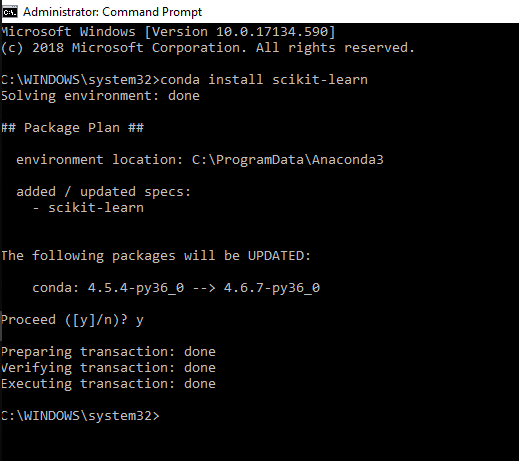
\includegraphics[scale=0.6]{figures/puad1.png}
\caption{Proses Instalasi}
\end{figure}
\begin{itemize}
\item ketik "pip install -U scikit-learn" untuk menggabungkan anaconda dan python
\end{itemize}
\begin{figure}[ht]
\centering
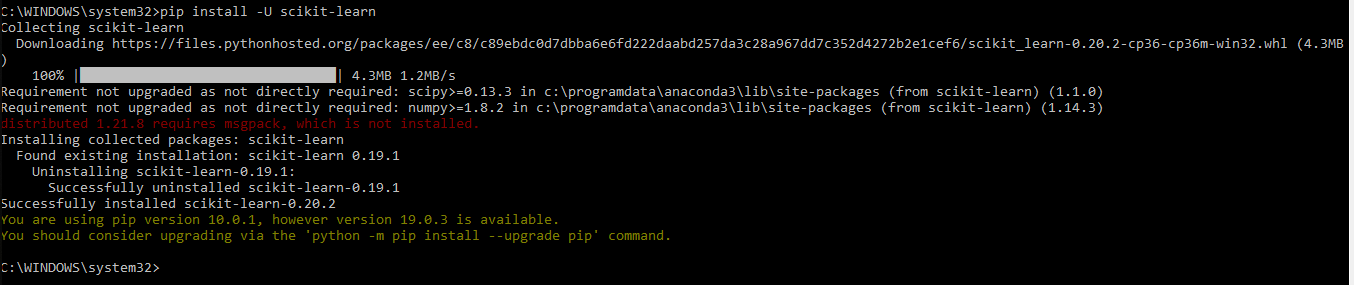
\includegraphics[scale=0.5]{figures/puad2.png}
\caption{Gabung Conda dan Python}
\end{figure}
\begin{itemize}
\item Setelah itu, kompilasi kode di dalam python dengan ketik "python", lalu "print('puad')" maka akan menghasilkan seperti gambar berikut.
\end{itemize}
\begin{figure}[ht]
\centering
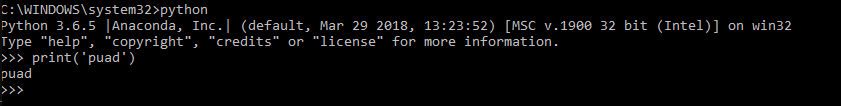
\includegraphics[scale=0.6 ]{figures/puad3.png}
\caption{Kompilasi Kode}
\end{figure}
\item Loading an Example Dataset
\begin{itemize}
\item Ketik perintah berikut "from sklearn import datasets" untuk mengimport dataset dari sklearn.
\end{itemize}
\begin{itemize}
\item ketik perintah "iris = datasets.load iris" untuk membuat variable iris yang berisi datasets.
\end{itemize}
\begin{itemize}
\item ketik perintah berikut"digits = datasets.load digits"untuk membuat variable digits yang berisi datasets, dan juga "print(digits.data) " untuk melihat isi data dari datasets seperti gambar 
\end{itemize}
\begin{figure}[ht]
\centering
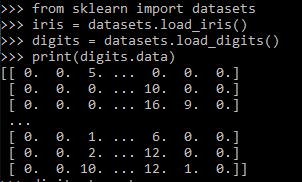
\includegraphics[scale=0.7]{figures/puad4.png}
\caption{Variable Digits}
\end{figure}
\begin{itemize}
\item kemudian  ketik "digits target"
\end{itemize}
\begin{figure}[ht]
\centering
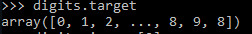
\includegraphics[scale=0.5]{figures/puad5.png}
\caption{}
\end{figure}
\begin{itemize}
\item kemudian  ketik "digits.images[0] "
\end{itemize}
\begin{figure}[ht]
\centering
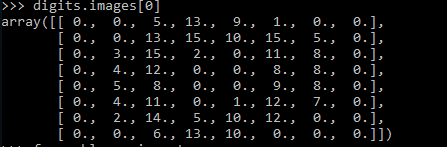
\includegraphics[scale=0.5]{figures/puad6.png}
\caption{}
\end{figure}
\begin{itemize}
\item kemudian  ketik "from sklearn import svm" dan kemudian clf = svm.SVC(gamma=0.001, C=100.) "
\item kemudian  ketik "clf.fit(digits.data[:-1], digits.target[:-1]) "
\end{itemize}
\begin{figure}[ht]
\centering
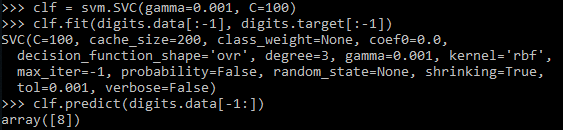
\includegraphics[scale=0.5]{figures/puad7.png}
\caption{}
\end{figure}
\begin{itemize}
\item kemudian  ketik "clf.predict(digits.data[-1:])"
\end{itemize}
\begin{figure}[ht]
\centering
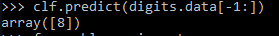
\includegraphics[scale=0.5]{figures/puad8.png}
\caption{}
\end{figure}
\begin{itemize}
\item kemudian  ketik "from sklearn import svm"
\item kemudian  ketik "from sklearn import datasets"
\item kemudian  ketik "clf = svm.SVC(gamma='scale')"
\item kemudian  ketik "iris = datasets.load(andeskore)iris()"
\item kemudian  ketik "X, y = iris.data, iris.target"
\item kemudian  ketik "clf.fit(X, y) "
\end{itemize}
\begin{figure}[ht]
\centering
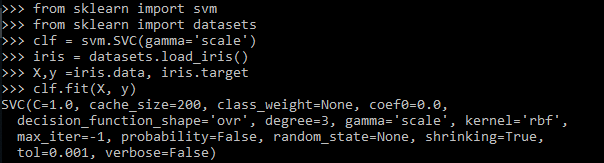
\includegraphics[scale=0.5]{figures/puad9.png}
\caption{}
\end{figure}
\begin{itemize}
\item kemudian  ketik "import pickle"
\item kemudian  ketik "s = pickle.dumps(clf)"
\item kemudian  ketik "clf2 = pickle.loads(s)"
\item kemudian  ketik "clf2.predict(X[0:1])"
\end{itemize}
\begin{figure}[ht]
\centering
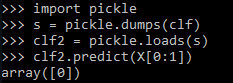
\includegraphics[scale=0.5]{figures/puad10.png}
\caption{}
\end{figure}
\begin{itemize}
\item kemudian  ketik " y[0]"
\end{itemize}
\begin{figure}[ht]
\centering
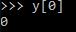
\includegraphics[scale=0.5]{figures/puad11.png}
\caption{}
\end{figure}
\begin{itemize}
\item kemudian  ketik "from joblib import dump, load"
\item kemudian  ketik "dump(clf, 'filename.joblib')"
\end{itemize}
\begin{figure}[ht]
\centering
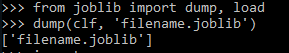
\includegraphics[scale=0.5]{figures/puad13.png}
\caption{}
\end{figure}
\begin{itemize}
\item conventions
\item ketikan "import numpy as np"
\item ketikan "from sklearn import random(andeskor)projection"
\item ketikan "rng = np.random.RandomState(0)"
\item ketikan "X = rng.rand(10, 2000)"
\item ketikan "X = np.array(X, dtype='float32')"
\item ketikan "X.dtype"
\item ketikan "transformer = random projection.GaussianRandomProjection"
\item ketikan "X new = transformer.fit transform(X)"
\item ketikan "X new.dtype"
\end{itemize}
\begin{figure}[ht]
\centering
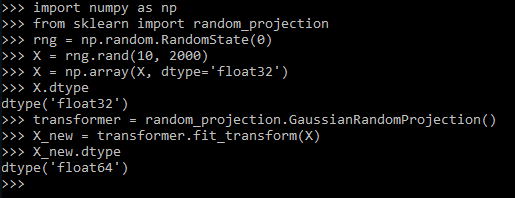
\includegraphics[scale=0.5]{figures/puad14.png}
\caption{}
\end{figure}
\item screenshoot eror
\begin{figure}[ht]
\centering
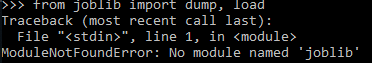
\includegraphics[scale=0.5]{figures/puad12.png}
\caption{}
\end{figure}
\item kode eror "no module named 'joblib'"
\item penanganannya instal joblib dengan mengetikan"conda instal -c anaconda joblib"
\end{enumerate}
>>>>>>> efee6eca5df5ee495d6544dd76ec774eee595c8a
=======
<<<<<<< HEAD
\section{Instalasi/Mhd Zulfikar Akram Nasution/1164081}
\begin{enumerate}
\item Menjelaskan Kode dari Learning and Predicting
\begin{itemize}
\item Pertama import file smv dari sklearn seperti pada gambar 1.12
\end{itemize}
\begin{figure}[ht]
\centering

\includegraphics[scale=0.9]{figures/2_1.png}
\caption{Import file svm}
\label{Import svm}
\end{figure}
\begin{itemize}
\item Kemudian buat variabel clf seperti pada gambar 1.13
\end{itemize}
\begin{figure}[ht]
\centering

\includegraphics[scale=0.9]{figures/2_2.png}
\caption{Buat variable Classifier}
\label{Variabel clf}
\end{figure}
\begin{itemize}
\item Lalu ketik kode berikut untuk meliat array baru dari syntax python [:-1] sepert padai gambar 1.14
\end{itemize}
\begin{figure}[ht]
\centering
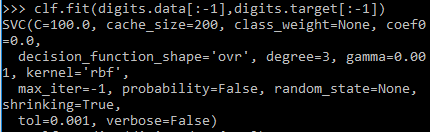
\includegraphics[scale=0.7]{figures/2_3.png}
\caption{Lihat array baru dengan syntac Python}
\label{Syntax python}
\end{figure}
\begin{itemize}
\item Selanjutnya ketikkan kode berikut untuk melihat penggolongan array seperti pada gambar 1.15
\end{itemize}
\begin{figure}[ht]
\centering
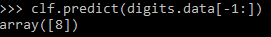
\includegraphics[scale=0.7]{figures/2_4.png}
\caption{Lihat classifier array}
\label{Classifier Array}
\end{figure}
\item Model Persistence
\begin{itemize}
\item Pertama Import dulu file dari sklearn
\end{itemize}
\begin{figure}[ht]
\centering
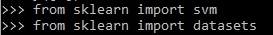
\includegraphics[scale=0.7]{figures/2_5.png}
\caption{Import file}
\end{figure}
\begin{itemize}
\item Kemudian buat variable classifier dengan gamma=scale
\end{itemize}
\begin{figure}[ht]
\centering

\includegraphics[scale=0.9]{figures/2_6.png}
\caption{Variable classifier}
\end{figure}
\begin{itemize}
\item Lalu buat variable iris dan (X,y)
\end{itemize}
\begin{figure}[ht]
\centering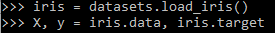
\includegraphics[scale=0.9]{figures/2_7.png}
\caption{Variable iris}
\end{figure}
\begin{itemize}
\item Selanjutnya kita akan melihat penyesuaian classifier
\end{itemize}
\begin{figure}[ht]
\centering
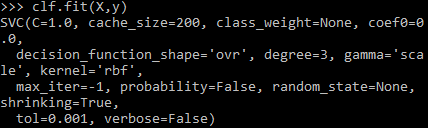
\includegraphics[scale=0.7]{figures/2_8.png}
\caption{Penyesuaian Classifier}
\end{figure}
\begin{itemize}
\item Kemudian import pickle untuk melihat hasil array dan hasil y
\end{itemize}
\begin{figure}[ht]
\centering
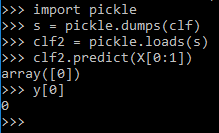
\includegraphics[scale=0.7]{figures/2_9.png}
\caption{Import Pickle}
\end{figure}
\item Conventions
\begin{itemize}
\item Pertama import numpy menjadi np serta import random projection
\end{itemize}
\begin{figure}[ht]
\centering
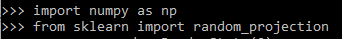
\includegraphics[scale=0.7]{figures/2_10.png}
\caption{Import numpy}
\end{figure}
\begin{itemize}
\item Kemudian buat variable rng dengan type random
\end{itemize}
\begin{figure}[ht]
\centering

\includegraphics[scale=0.7]{figures/2_11.png}
\caption{Variable rng}
\end{figure}
\begin{itemize}
\item Lalu buat variable X, dan lihat hasil rng random yang keluar
\end{itemize}
\begin{figure}[ht]
\centering
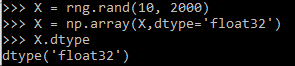
\includegraphics[scale=0.9]{figures/2_12.png}
\caption{Variable X dan hasil random}
\end{figure}
\begin{itemize}
\item Setelah itu buat variable transformer dengan type random
\end{itemize}
\begin{figure}[ht]
\centering
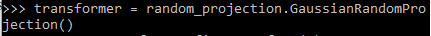
\includegraphics[scale=0.9]{figures/2_13.png}
\caption{Variable transformer random}
\end{figure}
\begin{itemize}
\item Berikutnya itu buat variable X new dengan type yang ada pada tranformer
\end{itemize}
\begin{figure}[ht]
\centering

\includegraphics[scale=0.9]{figures/2_14.png}
\caption{Variable X new type pada transformer}
\end{figure}
\begin{itemize}
\item Kemudian lihat hasil dari X new
\end{itemize}
\begin{figure}[ht]
\centering
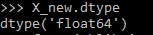
\includegraphics[scale=0.9]{figures/2_15.png}
\caption{Hasil dari X new type pada transformer}
\end{figure}
\item Screenshoot Error pada gambar 1.27
\begin{figure}[ht]
\centering
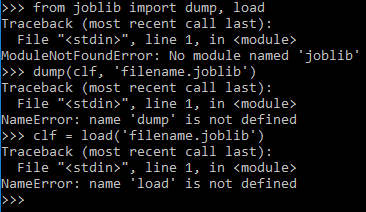
\includegraphics[scale=0.7]{figures/2_16.png}
\caption{Screenshoot Error}
\end{figure}
\item Kode yang error yaitu "joblib" karena belum ada library nya seperti pada gambar 1.28
\item Solusi dari masalah yang error seperti pada gambar 1.29
\begin{figure}[ht]
\centering
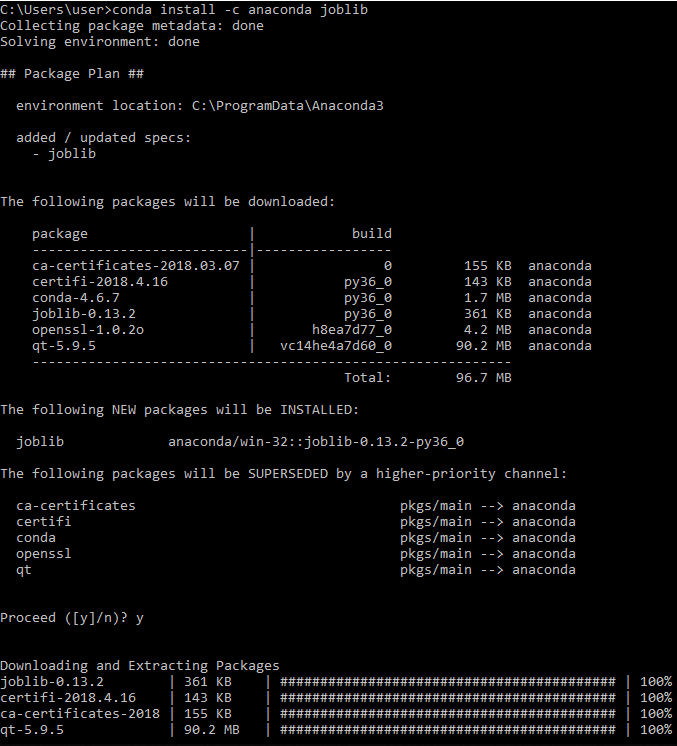
\includegraphics[scale=0.3]{figures/2_17.png}
\caption{Install Joblib}
\end{figure}
\begin{figure}[ht]
\centering
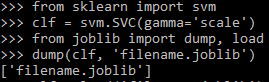
\includegraphics[scale=0.7]{figures/2_18.png}
\caption{Solusi Error}
\end{figure}


\end{enumerate}
=======
\subsection{Installasi}
\subsubsection{Loading an Example Datasets}
\begin{enumerate}
\item Loading an Example Dataset
\begin{itemize}
\item Ketik perintah berikut "from sklearn import datasets" untuk mengimport dataset dari file sklearn tadi.
\end{itemize}
\begin{figure}[ht]
\centering
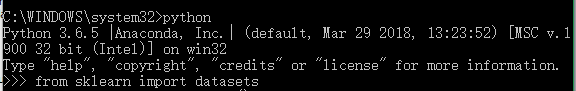
\includegraphics[scale=0.5]{figures/satu.png}
\caption{Perintah sklearn import datasets}
\label{Import Datasets}
\end{figure}
\begin{itemize}
\item Selanjutnya ketik perintah berikut ini untuk membuat variable iris yang berisi datasets.
\end{itemize}
\begin{figure}[ht]
\centering

\includegraphics[scale=0.9]{figures/dua.png}
\caption{Perintah Variabel Iris}
\label{Variable Iris}
\end{figure}
\begin{itemize}
\item Masukkan perintah ini untuk membuat variable digits yang berisi datasets, dapat juga untuk melihat isi data dari datasets tadi.
\end{itemize}
\begin{figure}[ht]
\centering
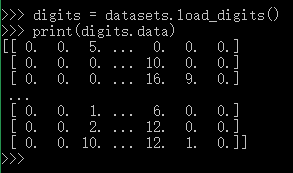
\includegraphics[scale=0.9]{figures/tiga.png}
\caption{Perintah Variabel Digits}
\label{Variable Digits}
\end{figure}
\end{enumerate}


\section{Learning and Predicting}
\begin{itemize}
\item from sklearn import svm ( pada baris berikut ini merupakan sebuah perintah untuk mengimport class svm dari package sklearn).
\item clf = svm.SVC (gamma=0.001, C=100.) (pada baris kedua ini clf sebagai estimator atau parameter, svm.SVC menjadi sebuah class, dan gamma sebagai parameter untuk menetapkan nilai secara manual)
\item clf.fit(digits.data[:-1], digits.target[:-1]) (pada baris ketiga ini clf sebagai estimator atau parameter, fit sebagai metode, digits.data sebagai item, [:-1] sebagai syntax pythonnya dan menampilkan outputannya)
\item clf.predict(digits.data[-1:])
\end{itemize}
\subsubsection{Model Presistence}
\begin{itemize}
\item from sklearn import svm
\item from sklearn import datasets
\item clf = svm.SVC(gamma='scale')
\item iris = datasets.load\_iris()
\item X, y = iris.data, iris.target
\item clf.fit(X, y)hasil
\item import pickle
\item s = pickle.dumps(clf)
\item clf2 = pickle.loads(s)
\item clf2.predict(X[0:1])hasil
\item y[0]hasil
\item from joblib import dump, load eror
\item dump(clf, 'filename.joblib')eror
\item clf = load('filename.joblib')eror
\end{itemize}
\subsubsection{Conventions}
\begin{enumerate}
\item Type Casting
\begin{itemize}
\item from sklearn import svm
\item from sklearn import random\_projection
\item rng = np.random.RandomState(0)
\item X = rng.rand(10, 2000)
\item X = np.array(X, dtype='float32')
\item X.dtype hasil
\item transformer = random\_projection.GaussianRandomProjection()
\item X\_new = transformer.fit\_transform(X)
\item X\_new.dtype hasil
\item from sklearn import datasets
\item from sklearn.svm import SVC
\item iris = datasets.load\_iris()
\item clf = SVC(gamma='scale')
\item clf.fit(iris.data, iris.target)hasil
\item list(clf.predict(iris.data[:3])) hasil
\item clf.fit(iris.data, iris.target\_names[iris.target]) hasil
\item list(clf.predict(iris.data[:3])) hasil
\end{itemize}
\item Refitting and Updating Parameters
\begin{itemize}
\item import numpy as np
\item from sklearn.svm import SVC
\item rng = np.random.RandomState(0)
\item X = rng.rand(100, 10)
\item y = rng.binomial(1, 0.5, 100)
\item X\_test = rng.rand(5, 10)
\item clf = SVC()
\item clf.set\_params(kernel='linear').fit(X, y) hasil
\item clf.predict(X\_test) hasil
\item clf.set\_params(kernel='rbf', gamma='scale').fit(X, y) hasil
\item clf.predict(X\_test) hasil
\end{itemize}
\item Multiclass vs. Multilabel Fitting
\begin{itemize}
\item from sklearn.svm import SVC
\item from sklearn.multiclass import OneVsRestClassifier
\item from sklearn.preprocessing import LabelBinarizer
\item X = [[1, 2], [2, 4], [4, 5], [3, 2], [3, 1]]
\item y = [0, 0, 1, 1, 2]
\item classif = OneVsRestClassifier(estimator=SVC(gamma='scale',random\_state=0))
\item classif.fit(X, y).predict(X) hasil
\item y = LabelBinarizer().fit\_transform(y)
\item classif.fit(X, y).predict(X) hasil
\item from sklearn.preprocessing import MultiLabelBinarizer
\item y = [[0, 1], [0, 2], [1, 3], [0, 2, 3], [2, 4]]
\item y = MultiLabelBinarizer().fit\_transform(y)
\item classif.fit(X, y).predict(X) hasil
\end{itemize}
\end{enumerate}

\section{Penanganan Error}
\begin{enumerate}
\item
Dibawah ini merupakan error yang ditemukan pada saat melakukan percobaan import.
\begin{figure}
\begin{center}
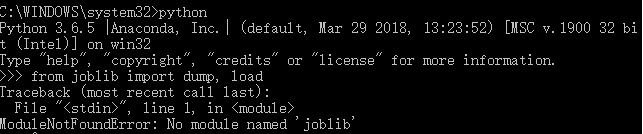
\includegraphics[scale=0.75]{figures/Error1.png}
\caption{Error Import}
\end{center}
\end{figure}
\item
Pada gambar diatas, terjadi error ketika sedang mengimport modul yang telah ditetapkan.
\item
Solusinya dapat dilakukan dengan berikut ini :\\
Error tadi terjadi akibat Library Joblib pada PC belum terinstall. Oleh sebab itu, install terlebih dahulu.
\item
Dengan membuka CMD (Admin), kemudian masukkan perintah "pip install joblib" dan tunggu sampai installasi berhasil seperti gambar berikut.
\begin{figure}
\begin{center}
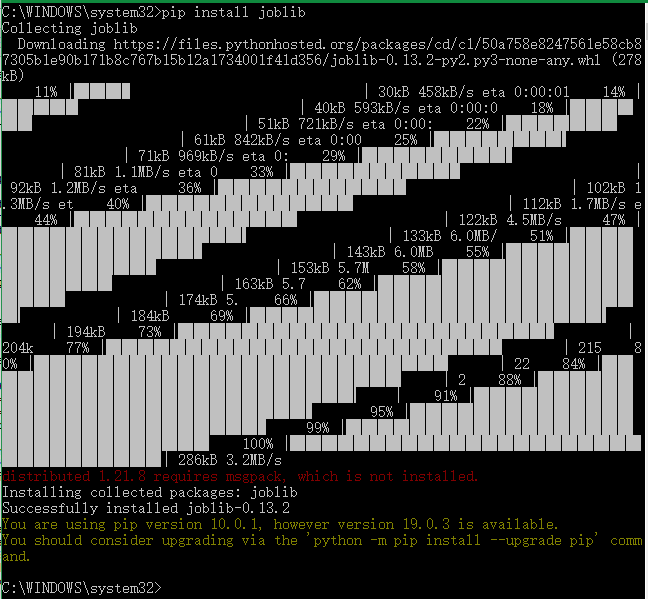
\includegraphics[scale=0.5]{figures/install2.png}
\caption{Install Library Joblib}
\end{center}
\end{figure}
\item
Ketika sudah terinstall, maka bisa dilakukan lagi import library joblib, dan hasilnya akan tampil seperti dibawah ini
\begin{figure}
\begin{center}
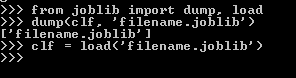
\includegraphics[scale=1]{figures/hasil3.png}
\caption{Berhasil Import Library Joblib}
\end{center}
\end{figure}
\end{enumerate}




>>>>>>> 
>>>>>>> f594df5d4cf2e0a7297e57a9c544d6f3fac837ab
>>>>>>> 2951ffb45da2a049bd0331edf27d34ed0e23f9f5

\chapter{Related Works}

Your related works, and your purpose and contribution which must be different as below.

\section{Mhd Zulfikar Akram Nasution/ 1164081}
\subsection{Teori}
\begin{enumerate}
\item Binary Classification atau diartikan kedalam bahasa indonesia yaitu Klasifikasi Biner adalah tugas dalam mengklarifikasikan elemen-elemen dari himpunan yang diberikan kedalam dua kelompok berdasarkan aturan klarifikasi. Pada ummnya klarifikasi biner akan jatuh ke dalam domain Supervised Learning dan dimana kasus khusus hanya memiliki dua kelas.
\begin{itemize}
\item  Contoh Binary Classification pada gambar 2.1
\end{itemize}
\begin{figure}[ht]
\centering
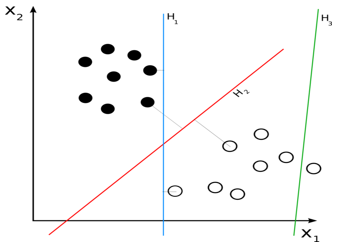
\includegraphics[scale=0.9]{figures/zulfikar/1.png}
\caption{Binary Classification}
\end{figure}

\item Supervised Learning, Unsupervised Learning, dan Clustering
\begin{itemize}
\item Supervised Learning
\end{itemize}
\par
Supervised learning adalah tugas pembelajaran mesin untuk mempelajari suatu fungsi yang memetakan input ke output berdasarkan contoh pasangan input-output. Ini menyimpulkan fungsi dari data pelatihan berlabel yang terdiri dari serangkaian contoh pelatihan. Dalam pembelajaran yang diawasi, setiap contoh adalah pasangan yang terdiri dari objek input (biasanya vektor) dan nilai output yang diinginkan (juga disebut sinyal pengawas). Contoh pada gambar 2.2
\begin{figure}[ht]
\centering
\includegraphics[scale=0.9]{figures/zulfikar/2.png}
\caption{Supervised Learning}
\end{figure}

\begin{itemize}
\item Unsupervised Learning
\end{itemize}
\par
Unsupervised Learning merupakan sebuah data yang belum ditentukan variabelnya jadi hanya berupa data saja. Dalam sebuah kasus Unsupervised Learning adalah aggap saja anda belum pernah membeli buku sama sekali dan pada suatu hari anda telah membeli buku dengan sangat banyak dalam kategori yang berbeda. Sehingga buku tersebut belum di kategorikan dan hanya berupa data buku saja. Coontoh seperti pada gambar 2.3
\begin{figure}[ht]
\centering
\includegraphics[scale=0.9]{figures/zulfikar/3.png}
\caption{Unsupervised Learning}
\end{figure}

\begin{itemize}
\item Clustering
\end{itemize}
\par
 Classtering merupakan sebuah proses untuk mengklasifikasikan sebuah data dalam satu parameter. Dalam kasus ini dapat dijelaskan ada beberapa orang yang memiliki kekuatan tubuh yang sehat dan kekuatan tubuh yang lemah. Parameter bagi orang yang memiliki tubuh yang kuat adalah orang yang terlihat bugar dan sehat maka dengan orang yang memiliki parameter adalah orang yang memiliki kekuatan tubuh yang kuat dan untuk kekuatan tubuh yang lemah adalah sebaliknya. Contoh seperti pada gambar 2.4
\begin{figure}[ht]
\centering
\includegraphics[scale=0.9]{figures/zulfikar/4.png}
\caption{Clustering}
\end{figure}

\item Evaluasi dan Akurasi
\par
 Evaluasi adalah tentang  bagaimana kita dapat mengevaluasi seberapa baik model bekerja dengan mengukur akurasinya. Dan akurasi akan didefinisikan sebagai persentase kasus yang diklasifikasikan dengan benar. Kita dapat menganalisis kesalahan yang dibuat oleh model, atau tingkat kebingungannya, menggunakan matriks kebingungan. Matriks kebingungan mengacu pada kebingungan dalam model, tetapi matriks kebingungan ini bisa menjadi sedikit sulit untuk dipahami ketika mereka menjadi sangat besar.

\item Cara Membuat dan Membaca Confusion Matrix
\begin{itemize}
\item Tentukan pokok permasalahan dan atributnya
\item Buat Decicion Tree
\item Buat Data Testing
\item Mencari nilai variabelnya misal a,b,c, dan d
\item Mencari nilai recall, percision, accuracy, dan error rate
\end{itemize}
\par contoh confusion matrix
	\begin{verbatim}
		Recall = 3/(1+3) = 0,75
		Percision = 3/(1+3 = 0,75
		Accuracy = (5+3)/(5+1+1+3) = 0,8
		Error Rate = (1+1)/(5+1+1+3) 0,2
	\end{verbatim}

\item Cara Kerja K-Fold Cross Validation
	\begin{itemize}
		\item Total instance dibagi menjadi N bagian.
		\item Fold yang pertama adalah bagian pertama menjadii testing data dan sisanya menjadi training data.
		\item Hitung akurasi berdasarkan porsi data tersebut dengan menggunakan persamaan.
		\item Fold yang ke dua adalah bagian ke dua menjadi testing data dan sisanya training data. 
		\item Hitung akurasi berdasarkan porsi data tersebut.
		\item Lakukan step secara berulang hingga habis mencapai fold ke-K.
		\item Terakhir hitung rata-rata akurasi K buah.
	\end{itemize}
\par
Berikut ilustrasi K-Fold Cross Validation seperti pada gambar 2.5
\begin{figure}[ht]
\centering
\includegraphics[scale=0.9]{figures/zulfikar/5.png}
\caption{K-Fold Cross Validation}
\end{figure}

\item Decision Tree
\par 
Decision Tree adalah sebuah metode pembelajaran yang digunakan untuk melakukan klarifikasi dan regresi. Decision Tree digunakan untuk membuat sebuah model yang dapat memprediksi sebuah nilai variabel target dengan cara mempelajari aturan keputusan dari fitur data. Contohnya seperti pada gambar 2.6 
\begin{figure}[ht]
\centering
\includegraphics[scale=0.9]{figures/zulfikar/6.png}
\caption{Decision Tree}
\end{figure}

\item Gain dan Entropi
\begin{itemize}
\item Gain adalah pengurangan yang diharapkan dalam enthropy. Dalam mechine learning, gain dapat digunakan untuk menentukan sebuah urutan atribut atau memperkecil atribut yang telah dipilih. Urutan ini akan membentuk decision tree. atribut gain dipilih yang paling besar.
\item  Entropi adalah ukuran ketidakpastian sebuah variabel acak sehingga dapat di artikan entropi adalah ukuran ketidakpastian dari sebuah atribut.
\end{itemize}
\par Contoh seperti pada gambar 2.7
\begin{figure}[ht]
\centering
\includegraphics[scale=0.9]{figures/zulfikar/7.png}
\caption{Gain dan Entropi}
\end{figure}
\end{enumerate}

\section{Mhd Zulfikar Akram Nasution/ 1164081}
\subsection{Scikit-Learn}

\begin{enumerate}
\item
\begin{verbatim}
	# load dataset (student mat pakenya)
	import pandas as pd
	lontong    = pd.read_csv('student-mat.csv', sep=';')
	len(lontong)
\end{verbatim}
\begin{figure}[ht]
\centering
\includegraphics[scale=0.9]{figures/lontong/1.png}
\caption{Load Dataset}
\end{figure}
\par
	Codingan pertama ini akan meload ( menampilkan ) data pada file yang ditentukan. Untuk codingan ini file yang dieksekusi ialah " student-mat.csv " . Secara jelasnya, dalam codingan dapat dilihat bahwa variabel lontong didefinisikan untuk pembacaan csv dari " lontong " dimana untuk pemisahnya yaitu separation berupa ; . Setelah itu variabel lontong di "print" dengan perintah menampilkan "len" panjang ataupun jumlah dan hasilnya berupa angka 649 . 

\item
\begin{verbatim}
	# generate binary label (pass/fail) based on G1+G2+G3 
	# (test grades, each 0-20 pts); threshold for passing is sum>=30
	lontong['pass'] = lontong.apply(lambda row: 1 if (row['G1']+row['G2']+row['G3']) 
											>= 35 else 0, axis=1)
	lontong = lontong.drop(['G1', 'G2', 'G3'], axis=1)
	lontong.head()
\end{verbatim}
\begin{figure}[ht]
\centering
\includegraphics[scale=0.6]{figures/lontong/2.png}
\caption{Generate Binary Label}
\end{figure}
\par
	Codingan kedua ini secara keseluruhan menampilkan  baris  G1, G2 dan G3 ( berdasarkan kriterianya ) untuk kolom PASS pada variabel lontong. Untuk lebih jelasnya, pada codingan terdapat pendefinisian pembacaan "lambda" ( panjang gelombang ) dari baris G1, G2 dan G3. Apabila row-row tersebut bernilai lebih dari 35 maka akan terdefinisikan angka "1" apabila tidak, maka akan terdefinisikan angka "0" pada kolom PASS ( sesuai permintaan awal ). Selanjutnya variabelnya di "print" sehingga menampilkan keluaran. Tidak lupa terdapat juga jumlah dari baris dan kolom yang terubah sesuai dengan baris yang dieksekusi.


\item
\begin{verbatim}
	# use one-hot encoding on categorical columns
	lontong = pd.get_dummies(lontong, columns=['sex', 'school', 'address', 
									'famsize', 
									'Pstatus', 'Mjob', 'Fjob', 
	                               'reason', 'guardian', 'schoolsup', 
								   'famsup', 'paid', 'activities',
	                               'nursery', 'higher', 'internet', 
									'romantic'])
	lontong.head()
\end{verbatim}
\begin{figure}[ht]
\centering
\includegraphics[scale=0.6]{figures/lontong/3.png}
\caption{Pemanggilan get dummies dari lontong}
\end{figure}
\par
	Secara keseluruhan, codingan ini mendefinisikan pemanggilan get dummies ke dalam variabel lontong. Di dalam get dummies sendiri akan terdefinisikan variabel lontong dengan kolom-kolom yang akan dieksekusi seperti school, address dll. Kemudian variabel tersebut di definisikan untuk mendapatkan kembalian berupa keluaran dari eksekusi perintah variabel lontong beserta dengan jumlah baris dan kolom data yang dieksekusi.

\item
\begin{verbatim}
	# shuffle rows
	lontong = lontong.sample(frac=1)
	# split training and testing data
	lontong_train = d[:500]
	lontong_test = d[500:]

	lontong_train_att = lontong_train.drop(['pass'], axis=1)
	lontong_train_pass = lontong_train['pass']

	lontong_test_att = lontong_test.drop(['pass'], axis=1)
	lontong_test_pass = lontong_test['pass']

	lontong_att = lontong.drop(['pass'], axis=1)
	lontong_pass = lontong['pass']

	# number of passing students in whole dataset:
	import numpy as np
	print("Passing: %d out of %d (%.2f%%)" % (np.sum(lontong_pass), len(lontong_pass), 
	       100*float(np.sum(lontong_pass)) / len(lontong_pass)))
\end{verbatim}
\begin{figure}[ht]
\centering
\includegraphics[scale=0.6]{figures/lontong/4.png}
\caption{Mendefinisikan pembagian data}
\end{figure}
\par
	Secara keseluruhan codingan ini difungsikan untuk mendefinisikan pembagian data yang berupa training dan testing data. Secara jelasnya pertama-tama variabel lontong akan mendefinisikan sampel yang akan digunakan ( berupa shuffle row ) . Nah kemudian masing2 parameter yaitu lontong train dan lontong test akan berjumlah 500 data ( telah dibagi untuk training dan testing ). Selanjutnya dilakukan pengeksekusian untuk kolom Pass, apabila sesuai dengan "axis=1" maka eksekusi fungsi berhasil. Selain itu juga disertakan jumlah dari peserta yang lolos dari semua nilai data setnya.

\item 
\begin{verbatim}
	# fit a decision tree
	from sklearn import tree
	soto = tree.DecisionTreeClassifier(criterion="entropy", max_depth=5)
	soto = soto.fit(lontong_train_att, lontong_train_pass)
\end{verbatim}
\begin{figure}[ht]
\centering
\includegraphics[scale=0.9]{figures/lontong/5.png}
\caption{Membuktikan pengujian}
\end{figure}
\par
	Secara keseluruhan, codingan ini hanya membuktikan pengujian dari Klasifikasi Decision Tree yang ada, apakah true atau tidak dan hasilnya true. Apabila dibahas secara lengkap maka pada codingan ini di definisikan library sklearn untuk mengimpor atau menampilkan tree. Variabel soto difungsikan untuk membaca klasifikasi decision tree dari tree itu sendiri dengan 2 parameternya yaitu kriteria="entropy" dan max depth=5. Maka selanjutnya variabel soto akan masuk dan terbaca dalam module fit dengan 2 parameter yaitu lontong trai att dan lontong train pass.

\item
\begin{verbatim}
	# visualize tree
	import graphviz
	dot_data = tree.export_graphviz(soto, out_file=None, label="all", 
									impurity=False, proportion=True,
	                                feature_names=list(lontong_train_att), 
									class_names=["fail", "pass"], 
	                                filled=True, rounded=True)
	graph = graphviz.Source(dot_data)
	graph
\end{verbatim}
\begin{figure}[ht]
\centering
\includegraphics[scale=0.3]{figures/lontong/6.png}
\caption{Gambaran decision tree}
\end{figure}
\par
	Codingan ini memberikan gambaran dari klasifikasi decision tree dari pengolahan parameter yang dieksekusi kedalam variabel soto. Tentunya dengan pemanfaatan library graphviz yang telah diimport dan difungsikan.

\item
\begin{verbatim}
	# save tree
	tree.export_graphviz(soto, out_file="student-performance.dot", 
						 label="all", impurity=False, 
						 proportion=True,
	                     feature_names=list(lontong_train_att), 
	                     class_names=["fail", "pass"], 
	                     filled=True, rounded=True)
\end{verbatim}
\begin{figure}[ht]
\centering
\includegraphics[scale=0.6]{figures/lontong/7.png}
\caption{Library Graphviz}
\end{figure}
\par
	Pada gambar 7 akan menampilkan yang terdapat pada Library Graphviz, apabila benar akan menampilkan hasil output seperti yang terdapat pada gambar.

\item
\begin{verbatim}
	soto.score(lontong_test_att, lontong_test_pass)
\end{verbatim}
\begin{figure}[ht]
\centering
\includegraphics[scale=0.9]{figures/lontong/8.png}
\caption{Menampilkan hasil perhitungan 2 parameter}
\end{figure}
\par
	Menampilkan hasil perhitungan dari kedua parameter yang terdapat pada code tersebut. Yang merupakan perhitungan hasil prediksi silang akan kemungkinan nilai di masa mendatang.

\item
\begin{verbatim}
	from sklearn.model_selection import cross_val_score
	kari = cross_val_score(soto, lontong_att, lontong_pass, cv=5)
	# show average score and +/- two standard deviations away 
	#(covering 95% of scores)
	print("Accuracy: %0.2f (+/- %0.2f)" % (kari.mean(), kari.std() * 2))
\end{verbatim}
\begin{figure}[ht]
\centering
\includegraphics[scale=0.6]{figures/lontong/9.png}
\caption{Mendefinisikan library sklearn}
\end{figure}
\par
	Kodingan tersebut mendefinisikan library sklearn model selection dan import cross val score. Dan kemudian variabel kari mengeksekusi fungsi cross val score(soto, lontong att, lontong pass, cv=5). Kemudian akan menampilkan nilai dari fungsi akurasinya.

\item 
\begin{verbatim}
	for max_depth in range(1, 20):
	    soto = tree.DecisionTreeClassifier(criterion="entropy", 
			max_depth=max_depth)
	    kari = cross_val_score(soto, lontong_att, lontong_pass, cv=5)
	    print("Max depth: %d, Accuracy: %0.2f (+/- %0.2f)" % 
				(max_depth, kari.mean(), kari.std() * 2)
			 )
\end{verbatim}
\begin{figure}[ht]
\centering
\includegraphics[scale=0.6]{figures/lontong/10.png}
\caption{Menampilkan hasil fungsi max depth dan accuracy}
\end{figure}
\par
	Pada gambar di atas kodingan nya berfungsi untuk menampilkan hasil dari fungsi Max Depth dan Accuraccy dari dari Decission Tree. Yaitu menmpilkan data dari angka 1-20.

\item
\begin{verbatim}
	depth_acc = np.empty((19,3), float)
	i = 0
	for max_depth in range(1, 20):
	    soto = tree.DecisionTreeClassifier(criterion="entropy", 
			max_depth=max_depth)
	    kari = cross_val_score(soto, lontong_att, lontong_pass, cv=5)
	    depth_acc[i,0] = max_depth
	    depth_acc[i,1] = kari.mean()
	    depth_acc[i,2] = kari.std() * 2
	    i += 1

	depth_acc
\end{verbatim}
\begin{figure}[ht]
\centering
\includegraphics[scale=0.6]{figures/lontong/11.png}
\caption{Menjelaskan variable kari}
\end{figure}
\par
	Dijelaskan bahwa variable kari akan menampilkan atau mendefinisikan nilai dari variabel score yang mana isi dari variable score yaitu soto, lontong att, lontong pass, cv=5. Yang mana hasil tampilan dari kodingannya adalah outputan seperti gambar 11.

\item 
\begin{verbatim}
	import matplotlib.pyplot as plt
	fig, ax = plt.subplots()
	ax.errorbar(depth_acc[:,0], depth_acc[:,1], yerr=depth_acc[:,2])
	plt.show()
\end{verbatim}
\begin{figure}[ht]
\centering
\includegraphics[scale=0.5]{figures/lontong/12.png}
\caption{Menjelaskan dan menampilkan gambar grafik}
\end{figure}
\par
	Pada gambar di atas dijelaskan bahwa pada library matplotlib akan menampilkan gambar grafik pada gambar 12 dari eksekusi fungsi ax.errorbar.

\end{enumerate}


\section{Penanganan Error}
Dari percobaan yang dilakukan di atas, error yang kita dapatkan di dokumentasikan dan di selesaikan(nilai 5 hari kedua):

\begin{enumerate}
	\item
ScreenShoot Error
\begin{figure}[ht]
\centering
\includegraphics[scale=0.3]{figures/lontong/13.png}
\caption{ScreenShoot Error}
\end{figure}
	\item
Tuliskan kode eror dan jenis errornya
\par
Error ini disebabkan karena pada direktori C tidak terdapat file tersebut. 
	\item
Solusi pemecahan masalah error tersebut
\begin{itemize}
\item 	Masuk ke folder dimana file dataset berada, dapat dilihat dibawah ini
\item 	Setelah diganti, jalankan kembali skrip tersebut pasti akan berhasil
\end{itemize}
\begin{figure}[ht]
\centering
\includegraphics[scale=0.3]{figures/lontong/14.png}
\caption{Penanganan Error}
\end{figure}

\end{enumerate}

\section{Same Topics}
Cite every latest journal with same topic
\subsection{Topic 1}
cite for first topic

\subsection{Topic 2}
if you have two topics you can include here to


\section{Same Method}
write and cite latest journal with same method

\subsection{Method 1}
cite and paraphrase method 1

\subsection{Method 2}
cite and paraphrase method 2 if you have more method please add new subsection.

\section{Teori/Jesron Marudut Hatuan/1164077}
\subsection{Binary classification dilengkapi ilustrasi gambar}
\begin{enumerate}
\item Binary classification yaitu berupa kelas-kelas positif dan kelas-kelas negatif. Klasifikasi biner adalah dikotomisasi yang diterapkan untuk tujuan praktis dan dalam banyak masalah klasifikasi biner praktis, kedua kelompok tidak simetris - daripada akurasi keseluruhan, proporsi relatif dari berbagai jenis kesalahan yang menarik. Misalnya, dalam pengujian medis, false positive (mendeteksi penyakit ketika tidak ada) dianggap berbeda dari false negative atau tidak mendeteksi penyakit ketika hadir.
\begin{figure}[ht]
\centering
\includegraphics[scale=0.5]{figures/1mrdt.jpg}
\caption{Klasifikasi Binari}
\label{contoh}
\end{figure}
\end{enumerate}


\subsection{ Pengertian Supervised Learning, Unsupervised Learning dan Clustering dan Illustrasi gambar}
\begin{enumerate}
\item Supervised learning adalah sesuatu pembelajaran yang terawasi yang dimana jika output yang diharapkan telah diketahui sebelum-sebelumnya. Biasanya Supervised Learning ini dilakukan dengan menggunakan data yang sudah ada. Pada metode ini, setiap pola yang diberikan kedalam jaringan saraf tiruan setelah diketahui outputnya. Satu pola input akan diberikan ke satu neuron pada lapisan-lapisan input. Pola-pola ini akan dirambatkan di sepanjang jaringan syaraf hingga sampai ke neuron pada lapisan output tersebut. Algoritma pembelajaran yang diawasi menganalisis data pelatihan dan menghasilkan fungsi yang disimpulkan, yang dapat digunakan untuk memetakan contoh-contoh baru. Skenario optimal akan memungkinkan algoritma menentukan label kelas dengan benar untuk instance yang tidak terlihat.
\begin{figure}[ht]
\centering
\includegraphics[scale=0.5]{figures/2mrdt.png}
\caption{Supervised Learning}
\label{contoh}
\end{figure}

\item Unsupervised learning merupakan sebuah pembelarajan yang tidak terawasi dimana tidak memerlukan target output. Pada metode ini tidak dapat ditentukan hasil seperti apa yang diharapkan selama proses pembelajaran, nilai bobot yang disusun dalam proses range tertentu tergantung pada sebuah nilai output yang telah diberikan. Tujuan metode unsupervised learning ini agar dapat mengelompokkan unit-unit yang hampir sama dalam satu area tertentu. Pembelajaran ini biasanya sangat cocok untuk klasifikasi pola-pola. Contohny algoritma jaringan saraf tiruan yang menggunakan metode unsupervised ini merupakan competitive, kohonen, LVQ(Learning Vector Quantization), neocognitron.
\begin{figure}[ht]
\centering
\includegraphics[scale=0.5]{figures/3mrdt.png}
\caption{Unsupervised Learning}
\label{contoh}
\end{figure}
\item Analisis Cluster adalah sebuah teknik statistika yang dapat berguna untuk mengelompokkan sebuah objek-objek ataupun variable-variable ke dalam beberapa grup tertentu dimana pada setiap objek atau variable yang telah terbentuk mempunyai sifat dan karakteristik yang berdekatan tersebut.Gagasan populer mengenai cluster termasuk kelompok dengan jarak kecil antara anggota cluster, area padat ruang data, interval atau distribusi statistik tertentu. Clustering karena itu dapat dirumuskan sebagai masalah optimasi multi-objektif. Algoritma pengelompokan dan pengaturan parameter yang sesuai (termasuk parameter seperti fungsi jarak yang akan digunakan, ambang kepadatan atau jumlah cluster yang diharapkan) tergantung pada set data individual dan penggunaan hasil yang dimaksudkan.
\begin{figure}[ht]
\centering
\includegraphics[scale=0.5]{figures/4mrdt.png}
\caption{Cluster}
\label{contoh}
\end{figure}
\end{enumerate}

\subsection{Evaluasi dan akurasi dan Illustrasi gambar}
\begin{enumerate}
\item Evaluasi merupakan suatu langkah bagaimana agar dapat mengevaluasi seberapa baik model bekerja dengan cara mengukur tingkat akurasinya. Dan akurasi tersebut akan didefinisikan menjadi sebuah persentasi studi kasus yang telah diklasifikasikan dengan benar. Dapat juga untuk menganalisis kesalahan yang dibuat oleh sebuah model, atau tingkat kebingungannya, menggunakan matriks kebingungan. Matriks kebingungan mengacu pada sebuah kebingungan dalam model, tetapi matriks kebingungan ini bisa menjadi sedikit sulit untuk dipahami ketika mereka menjadi sangat besar.
\begin{figure}[ht]
\centering
\includegraphics[scale=0.5]{figures/5mrdt.png}
\caption{ Evaluasi dan Akurasi}
\label{contoh}
\end{figure}
\end{enumerate}

\subsection{ Cara membuat dan membaca confusion matrix, buat confusion matrix }
\begin{enumerate}
\item Cara membuat dan membaca confusion matrix :
\begin{itemize}
\item 1)	Menentukan pokok sebuah permasalahan dan atribut-atributnya, misal gaji dan listik.
\item 2)	Buat pohon keputusan
\item 3)	Lalu data testingnya
\item 4)	Lalu mencari nilai a, b, c, dan d. Semisal a = 5, b = 1, c = 1, dan d = 3.
\item 5)	Selanjutnya mencari nilai recall, precision, accuracy, serta dan error rate.
\end{itemize}
\item Berikut adalah contoh dari confusion matrix :
\begin{itemize}
\item Recall =3/(1+3) = 0,75
\item Precision = 3/(1+3) = 0,75
\item Accuracy =(5+3)/(5+1+1+3) = 0,8
\item Error Rate =(1+1)/(5+1+1+3) = 0,2
\end{itemize}
\end{enumerate}

\subsection{Membuat cara K-fold cross validation bekerja dengan gambar ilustrasi}
\begin{enumerate}
\item Cara kerja K-fold cross validation :
\begin{itemize}
\item 1)	Total instance dibagi menjadi N bagian.
\item 2)	Fold yang pertama adalah bagian pertama menjadi data uji (testing data) dan sisanya menjadi training data.
\item 3)	Lalu hitung akurasi berdasarkan porsi data tersebut dengan menggunakan persamaan.
\item 4)	Fold yang ke dua adalah bagian ke dua menjadi data uji (testing data) dan sisanya training data. 
\item 5)	Kemudian hitung akurasi berdasarkan porsi data tersebut.
\item 6)	Dan seterusnya hingga habis mencapai fold ke-K.
\item 7)	Terakhir hitung rata-rata akurasi K buah.
\end{itemize}
\begin{figure}[ht]
\centering
\includegraphics[scale=0.5]{figures/6mrdt.png}
\caption{K-fold cross validation}
\label{contoh}
\end{figure}
\end{enumerate}

\subsection{Decision tree dengan gambar ilustrasi}
\begin{enumerate}
\item Decision Tree dalah metode pembelajaran yang diawasi non-parametrik yang digunakan untuk mengklasifikasi dan regresi. Tujuannya adalah untuk membuat model yang memprediksi nilai variabel target dengan mempelajari aturan keputusan sederhana yang disimpulkan dari fitur data. Decision tree memadukan antara eksplorasi data dan sebuah pemodelan, sehingga sangat bagus sebagai langkah awal dalam proses pemodelan bahkan ketika dijadikan menjadi sebuah model akhir dari beberapa teknik lain.\\
\begin{figure}[ht]
\centering
\includegraphics[scale=0.5]{figures/7mrdt.png}
\caption{Decision Tree}
\label{contoh}
\end{figure}
\end{enumerate}

\subsection{Information Gain dan entropi dengan gambar ilustrasi}
\begin{enumerate}
\item Information gain dapat didasarkan kepada penurunan entropi setelah dataset yang sebelumnya dapat dibagi pada atributnya. Untuk membangun sebuah decision tree, merupakan cara agar semua tentang menemukan atribut yang mengembalikan perolehan informasi tertinggi dari yang lainnya.
\begin{figure}[ht]
\centering
\includegraphics[scale=0.5]{figures/8mrdt.png}
\caption{Information gain}
\label{contoh}
\end{figure}
\item Entropi adalah cara untuk mengukur keacakan dalam sebuah sistem informasi yang sedang diproses. Semakin tinggi entropi, mka hasilnya semakin sulit untuk menarik kesimpulan dari informasi tersebut. Melempar koin merupakan salah satu contoh tindakan yang memberikan informasi yang random. Untuk koin yang tidak memiliki afinitas untuk kepala atau ekor, hasil dari sejumlah lemparan sulit diprediksi. Mengapa? Karena tidak ada hubungan antara membalik dan hasilnya. Inilah inti dari entropi.
\begin{figure}[ht]
\centering
\includegraphics[scale=0.5]{figures/9mrdt.png}
\caption{Entropi}
\label{contoh}
\end{figure}
\end{enumerate}


\subsection{Scikit-learn}
\begin{enumerate}
\item Penjelasan kodingan ini akan menampilkan data pada file yang ditentukan. Untuk codingan ini file yang dieksekusi untuk digunakan ialah student-mat.csv. Dalam codingan dapat dilihat bahwa variabel Rambutan dapat  didefinisikan untuk pembacaan file csv dari  Durian  dimana untuk pemisahnya yaitu separation berupa ; . Setelah itu variabel Rambutan di tampilkan dengan perintah menampilkan len panjang ataupun jumlah dan hasilnya berupa angka 395 . 
\begin{figure}[ht]
\centering
\includegraphics[scale=0.5]{figures/no1.png}
\caption{Load Dataset}
\label{Hasil}
\end{figure}
\end{enumerate}

\begin{enumerate}
\item Kodingan berikut berguna untuk menampilkan setiap baris  G1, G2 dan G3 untuk kolom PASS pada variabel Rambutan. Untuk lebih jelasnya, pada kodingan terdapat pendefinisian pembacaan lamda ( panjang gelombang ) dari baris G1, G2 dan G3. Apabila row-row tersebut bernilai lebih dari 35 maka akan terdefinisikan angka 1 apabila tidak, maka akan terdefinisikan angka 0 pada kolom PASS ( sesuai permintaan awal ). Selanjutnya variabelnya di ditampilkan sehingga menampilkan keluaran. Tidak lupa terdapat juga jumlah dari baris dan kolom yang terubah sesuai dengan baris yang dieksekusi.
\begin{figure}[ht]
\centering
\includegraphics[scale=0.5]{figures/no2.png}
\caption{Generate Binary label}
\label{Hasil}
\end{figure}
\end{enumerate}

\begin{enumerate}
\item Kodingan berikut mendefinisikan pemanggilan get dummies dari Durian dalam variabel Rambutan. Di dalam get dummies sendiri akan terdefinisikan variabel Rambutan dengan kolom-kolom yang akan dieksekusi seperti school, address dll. Kemudian variabel tersebut diartikan untuk mendapatkan kembalian berupa keluaran dari eksekusi perintah variabel Rambutan beserta dengan jumlah baris dan kolom data yang dieksekusi.
\begin{figure}[ht]
\centering
\includegraphics[scale=0.5]{figures/no3.png}
\caption{Use one-hot encoding}
\label{Hasil}
\end{figure}
\end{enumerate}

\begin{enumerate}
\item Kodingan ini dipakai untuk mengartikan pembagian data yang berupa training dan testing data. Pertama-tama variabel Rambutan akan mengartikan sampel yang akan digunakan. Selanjutnya masing-masing parameter yaitu Rambutan train dan Rambutan test akan berjumlah 500 data. Selanjutnya dilakukan pengeksekusian untuk kolom Pass, apabila sesuai dengan axis=1 maka eksekusi fungsi berhasil. Selain itu juga disertakan jumlah dari peserta yang lolos dari semua nilai data setnya.  
\begin{figure}[ht]
\centering
\includegraphics[scale=0.5]{figures/no4.png}
\caption{Shuffle rows}
\label{Hasil}
\end{figure}
\end{enumerate}

\begin{enumerate}
\item Kodingan ini dapat membuktikan pengujian dari Klasifikasi Decision Tree yang ada, apakah true atau tidak dan hasilnya true. Pada kodingan ini di definisikan library sklearn untuk mengimpot atau menampilkan tree. Variabel timun difungsikan untuk membaca klasifikasi decision tree dari tree itu sendiri dengan 2 parameternya yaitu kriteria=entropy dan max depth=5. Maka selanjutnya variabel timun akan masuk dan terbaca dalam module fit dengan 2 parameter yaitu Rambutan trai att dan Rambutan train pass.
\begin{figure}[ht]
\centering
\includegraphics[scale=0.5]{figures/no5.png}
\caption{Fit a Decision tree}
\label{Hasil}
\end{figure}
\end{enumerate}

\begin{enumerate}
\item Penjelasan kodingan ini memberikan gambaran dari klasifikasi decision tree yaitu pengolahan parameter yang dieksekusi kedalam variabel timun. Tentunya dengan pemanfaatan library graphviz yang telah diimport dan difungsikan.
\begin{figure}[ht]
\centering
\includegraphics[scale=0.5]{figures/no6.png}
\caption{Visualize tree}
\label{Hasil}
\end{figure}
\end{enumerate}

\begin{enumerate}
\item Penjelasan kodingan ini membahas tentang penyimpanan tree dari library graphviz yang dieksekusi bersamaan dengan variabel timun dan parameter lainnya. Dilakukan pengecekan dan pengujian apakah klasifikasi decision treenya dapat berjalan atau tidak. Apabila tidak berjalan, maka akan terjadi error, namun kodingan ini berfungsi.
\begin{figure}[ht]
\centering
\includegraphics[scale=0.5]{figures/no7.png}
\caption{Save tree}
\label{Hasil}
\end{figure}
\end{enumerate}

\begin{enumerate}
\item Penjelasan kodingan ini membaca skore dari variabel timun dimana terdapat 2 parameter yang dihitung dan diuji yaitu Rambutan test att dan Rambutan test pass. Untuk hasilnya sendiri mengapa berupa angka, dikarenakan pada parameter yang dieksekusi memang memiliki data sehingga dieksekusi dan menghasilkan keluaran dari score tersebut.
\begin{figure}[ht]
\centering
\includegraphics[scale=0.5]{figures/no8.png}
\caption{Score}
\label{Hasil}
\end{figure}
\end{enumerate}

\begin{enumerate}
\item Penjelasan kodingan ini membahas mengenai pengkesekusian fungsi dan variabel dari library yang didefinisikan dan yang diimport. Penjelasan lebih jelasnya ialah kodingan ini mendefinisikan library sklearn.model.selection kemudian mengimport cross val score. Kemudian variabel score mendefinisikan cross val score yang telah diimport tadi dengan 4 parameter yaitu timun, Rambutan att, Rambutan pass dan cv=5 untuk dieksekusi. Setelah semua pemrosesan tersebut maka hasil yang di tampilkan ialah rata-rata perhitungan dari variabel score dimana dan standar dari plus minusnya tentunya dengan ketentuan parameter Accuracy .
\begin{figure}[ht]
\centering
\includegraphics[scale=0.5]{figures/no9.png}
\caption{Show Averange score}
\label{Hasil}
\end{figure}
\end{enumerate}

\begin{enumerate}
\item Penjelasan kodingan ini mendefinisikan max depth dalam jarak angka antara parameter 1 dan 20. Variabel timun mendefinisikan klasifikasi decision tree dengan 2 parameter. Kemudian variabel score mengeksekusi parameter lainnya yaitu seperti timun, Rambutan att, Rambutan pass dan cv=5 ) . Hasil yang ditampilkan ialah dari max depth, accuracy dan plus minusnya dan akhirnya hasil outputannya keluar.
\begin{figure}[ht]
\centering
\includegraphics[scale=0.5]{figures/no10.png}
\caption{Max depth}
\label{Hasil}
\end{figure}
\end{enumerate}

\begin{enumerate}
\item Kodingan ini mengartikan bahwa variabel depth\_acc akan mengeksekusi empty dari importan library numphy yang dinamakan np dengan 2 parameter yaitu 19,3 dan float. i didefinisikan dengan angka 0 kemudian untuk perhitungan jarak max depth diantara parameter 1 dan 20. Variabel np mengartikan klasifikasi decision tree dengan 2 parameter. Setelah itu, variabel score mendefinisikan variabel depth\_acc dengan i dan 0, variabel kedua dari depth\_acc dengan i dan 1 serta variabel ketiga dari depth\_acc dengan i dan 2, maka pengeksekusian akhir bahwa variabel i akan ditambah dengan angka 1 untuk hasil akhirnya. Keluarannya akan berupa array dari perhitungan parameter dan variabel yang telah didefinisikan sebelumnya.
\begin{figure}[ht]
\centering
\includegraphics[scale=0.5]{figures/no11.png}
\caption{Depth Acc}
\label{Hasil}
\end{figure}
\end{enumerate}

\begin{enumerate}
\item Kodingan mendefinisikan pemanggilan dari library matplotlib.pyplot sebagai salak sehingga nanti hasilnya akan berbentuk gambar grafik/gelombang. Untuk variabel fig dan ax akan mendefinisikan subplots dari salak. Setelah itu ketentuan dari parameter depth acc = 0, depth acc = 1 dan depth acc 2. Selanjutnya untuk menampilkan gelombang maka panggil variabel salak dengan perintah show.
\begin{figure}[ht]
\centering
\includegraphics[scale=0.5]{figures/no12.png}
\caption{Import}
\label{Hasil}
\end{figure}
\end{enumerate}

\subsection{Penanganan Eror}
\begin{enumerate}
\item Kodingan eror dan jenis erornya : sebenarnya tidak terdapat eror pada codingan ini namun saat pertama kali di run current cell codingan ini akan eror dan tidak keluar outputannya dikarenakan library graphviz sebelumnya tidak ditemukan atau belum di install terlebih dahulu.
\subitem 
\begin{verbatim}
import graphviz
dot_data = tree.export_graphviz(buahapel, out_file=None, label="all", impurity=False, proportion=True,
                                feature_names=list(buahpir_train_att), class_names=["fail", "pass"], 
                                filled=True, rounded=True)
graph = graphviz.Source(dot_data)
graph
\end{verbatim}
\item Solusi pemecahan masalah eror tersebut yaitu dengan cara menginstall terlebih dahulu library graphviznya pada anaconda prompt atau command prompt dengan perintah conda install graphviz setelah itu run kembali codingan No 8 maka akan muncul outputan atau tampilan keluarannya.
\end{enumerate}

 
\chapter{Methods}

\section{The data}
PLease tell where is the data come from, a little brief of company can be put here.
\section {Puad Hamdani/ 1164084}
\subsection {Teori}
\begin{enumerate}
\item Random Forest
\par
Merupakan classifier yang terdiri dari banyak pohon keputusan dan melakukan klasifikasi berdasarkan keluaran dari hasil klasifikasi setiap pohon keputusan anggota
\begin{figure}[ht]
\centering
\includegraphics[scale=0.5]{figures/111.JPG}
\caption{Random Forest}
\end{figure}
\item Cara membaca dataset kasus
\begin{itemize}
\item Buka aplikasi spyder untuk membuka dan membaca kodingan dataset
\item Kemudian buat  variable imgatt untuk memasukkan atribut label
\item Lalu uji coba kodingan untuk mengetahui apa hasil dari dataset tersebut
\item imgatt.head() untuk melihat sebagian data awal
\item .shape untuk melihat jumlah data
\item .pivot untuk merubah atribut menjadi kolom
\par
Dengan menguji coba kodingan yang ada pada spyder untuk membaca data set.
\end{itemize}
\item Cross Validation
\par 
Cross Validation adalah teknik validasi model untuk menilai bagaimana hasil analisis statistik (model) akan digeneralisasi ke kumpulan data independen. terutama digunakan dalam pengaturan di mana tujuannya adalah prediksi, dan orang ingin memperkirakan seberapa akurat model prediksi akan dilakukan dalam praktek
\item Arti 44 persen pada RF, 27 persen pada Decission Tree, dan 29 persen pada SVM.
\begin{itemize}
\item Merupakan akurasi dari sebuah pohon keputusan untuk menunjukkan hasil keputusan dengan klasifikasi dari dataset yang ada.
\end{itemize}
\item Confusion Matrix
\begin{itemize}
\item Import confusion matrix
\item Plot confusion matrix
\item Lalu sesuaikan plotnya
\item Setelah itu plot kembali
\end{itemize}
\item Voting
\par
Voting Merupakan metode untuk menentukan keputusan dalam suatu suatu pemilihan, berdasarkan pendapat per orang, dan keputusan ditentukan berdasarkan pemilih terbanyak

\end{enumerate}
\section{Method 1}
Definition, steps, algoritm or equation of method 1 and how to apply into your data
\section{Method 2}
Definition, steps, algoritm or equation of method 2 and how to apply into your data

\chapter{Experiment and Result}
brief of experiment and result.
\section{Experiment}
Please tell how the experiment conducted from method.

\section{Result}
Please provide the result of experiment

\section{Mhd Zulfikar Akram Nastuion / 1164081}
\subsection{Teori}
\begin{enumerate}
\item Klasifikasi Teks
\par
Klasifikasi teks adalah sebuah proses untuk menempatkan dokumen teks ke dalam suatu kategori berdasarkan isi dari teks tersebut. 
\item Kenapa klasifikasi bunga tidak bisa menggunakan machine learning
\par
Klasifikasi bunga tidak dapat digunakan pada machine learning karena terdapat masalah, yaitu apabila kita memasukkan suatu inputan yang sama tetapi outputnya berbeda.
\item  Teknik pembelajaran mesin pada teks pada kata-kata yang digunakan di Youtube
\par
Penggunaan machine learning pada Youtube contohnya ada pada saat kita sedang melakukan pencarian judul, nama dan lainnya maka youtube akan menampilkan apa yang kita cari, kemudian saat kita sedang melihat youtube, dibagian kanan video terlihat ada tampilan video yang berkaitan dengan apa yang kita cari atau kita ketikkan di tempat pencarian terbebut.
\item Vectorisasi Data
\par
Vektorisasi data adalah sebuah proses pembagian dan pemecahan data kemudian dilakukan perhitungan datanya.
\item Bag of Words
\par
Bag of words adalah sebuah proses penyederhanaan yang digunakan dalam pengambilan informasi.
\item TF-IDF
\par
TF-IDF adalah sebuah metode untuk menghitung beberapa kata yang muncul dari setiap kata yang paling umum digunakan.
\end{enumerate}

\subsection{Praktek}
\begin{enumerate}
\item Membuat aplikasi sederhana meggunakan pandas
\begin{figure}[ht]
\centering
\includegraphics[scale=0.7]{figures/pandas/4_1.png}
\caption{Aplikasi sederhana pandas}
\end{figure}
\begin{itemize}
\item Baris 1: Memanggil library pandas sebagai coba1
\item Baris 2: Membaca dataset Indian Liver Patient Dataset
\item Baris 3: Dataset.head menampilkan jumlah baris pada dataset
\item Baris 4: Dataset.shape menampilkan jumlah kolom pada dateset
\par Hasilnya seperti gambar 4.1
\end{itemize}
\item Membuat aplikasi sederhana meggunakan pandas
\begin{figure}[ht]
\centering
\includegraphics[scale=0.9]{figures/pandas/4_2.png}
\caption{Hasil aplikasi sederhana pandas}
\end{figure}
\item Membuat aplikasi sederhana menggunakan pandas, dan membuat data dummy sebanyak 500 baris dan melakukan data load ke data frame panda
\begin{figure}[ht]
\centering
\includegraphics[scale=0.9]{figures/pandas/4_3.png}
\caption{Membuat data dummy sebanyak 500}
\end{figure}
\begin{itemize}
\item Baris 1: Membagi data set ILPD dari 500 data menjadi data train menjadi 450 data.
\item Baris 2: Membagi data set ILPD dari sisa pembagian data train menjadi data test menjadi 50 data.
\end{itemize}
\par Hasilnya seperti pada gambar 4.3
\begin{figure}[ht]
\centering
\includegraphics[scale=0.9]{figures/pandas/4_4.png}
\caption{Hasil membuat data dummy sebanyak 500}
\end{figure}
\item  Vektorisasi dan Klasifikasi Data Dengan Decission Tree
\begin{itemize}
\item Berikut ini adalah hasil dari NPM mod 4
\end{itemize}
\begin{figure}[ht]
\centering
\includegraphics[scale=0.9]{figures/pandas/4_5.png}
\caption{NPM mod 4}
\end{figure}
\begin {itemize}
\item Vektorisasi seperti pada gambar 4.4
\end{itemize}
\begin{figure}[ht]
\centering
\includegraphics[scale=0.9]{figures/pandas/4_6.png}
\caption{Vektorisasi}
\end{figure}
\begin {itemize}
\item Klasifikasi data dengan desision Tree seperti pada gambar 4.5
\end{itemize}
\begin{figure}[ht]
\centering
\includegraphics[scale=0.7]{figures/pandas/4_7.png}
\caption{Klasifikasi dengan Tree}
\end{figure}
\begin{itemize}
\item Dalam in 48 impor tree dari sklearn. Dan mendefinisikan variabel clftree untuk memanggil Decission Tree Classifier dan melakukan fit atau pengujian.
\item clftree.score memunculkan akurasi prediksi yang dilakukan terhadap clftree
\end{itemize}
\item Klasifikasi SVM seperti pada gambar 4.6
\begin{figure}[ht]
\centering
\includegraphics[scale=0.9]{figures/pandas/4_8.png}
\caption{Klasifikasi SVM}
\end{figure}
\begin{itemize}
\item Import SVM dari  sklearn
\item Melakukan fit dari train att dan train label atau disebut denga pengujian
\item Mendefinisikan variabel clfsvm untuk melakukan prediksi dataset Youtube LMFAO dengan SVM. Dan akan muncul hasil prediksinya 
\end{itemize}
\item Klasifikasi decision tree seperti pada gambar 4.7
\begin{figure}[ht]
\centering
\includegraphics[scale=0.9]{figures/pandas/4_7.png}
\caption{Klasifikasi decision tree}
\end{figure}
\begin{itemize}
\item Import tree dari  sklearn
\item Melakukan fit dari train att dan train label atau disebut denga pengujian
\item  clftree.score memunculkan akurasi prediksi yang dilakukan terhadap clftree 
\end{itemize}
\item Matplotlib seperti pada gambar4.8
\begin{figure}[ht]
\centering
\includegraphics[scale=0.9]{figures/pandas/4_9.png}
\caption{Matplotlib}
\end{figure}
\par Fungsi ini mencetak dan memplot Confussion Matrix. Normalisasi dapat diterapkan dengan mengatur `normalize = True`. Ada Confussion Matrik menggunakan normalisasi dan ada confussion matrik tidak menggunakan normalisasi.
\item Menjelaskan program cross validation seperti pada gambar 4.9
\begin{figure}[ht]
\centering
\includegraphics[scale=0.9]{figures/pandas/4_10.png}
\caption{Cross Validation}
\end{figure}
\par Variable score akan melakukan cross validation pada variable clf, train att, train label. Variabel scores akan menghitung nilai rata-rat menggunakan function mean. Dan scores menghitung standar deviasi dari data yang diberikan. Hasilnya seperti pada gambar 4.10
\begin{figure}[ht]
\centering
\includegraphics[scale=0.9]{figures/pandas/4_11.png}
\caption{Hasil Cross Validation}
\end{figure}
\item Proses pengamatan komponen seperti pada gambar 4.11
\begin{figure}[ht]
\centering
\includegraphics[scale=0.9]{figures/pandas/4_12.png}
\caption{Pengamatan komponen}
\end{figure}
\par Pada gambar tersebut merupakan kodingan dan hasil dari macfeatures, num estimators dan accuracy.
\end{enumerate}
\chapter{Conclusion}
brief of conclusion

\section{Conclusion of Problems}
Tell about solving the problem

\section{Conclusion of Method}
Tell about solving using method

\section{Conclusion of Experiment}
Tell about solving in the experiment

\section{Conclusion of Result}
tell about result for purpose of this research.
<<<<<<< HEAD
\section{Puad Hamdani/1164084}
\subsection{Teori}
\begin{enumerate}
\item Vektorisasi Kata-Kata
\begin{itemize}
\item Penjelasan :
\par Alasan mengapa kata-kata harus dilakukan vektorisasi yaitu dikarenakan mesin hanya mampu membaca data dengan bentuk angka. Berdasarkan hal tersebut,diperlukan vektorisasi kata atau mengubah kata menjadi bentuk vektor agar mesin  paham apa yang kita maksudkan dan dapat memproses perintah dengan benar.
\item Mengapa Dimensi Dari Vektor Dataset Google Bisa Mencapai 300


\item  Penjelasan :
\par Dimensi dari Vektor Dataset Google Mencapai 300 karena  pada masing-masing objek yang terdapat pada dataset akan memiliki identitasnya tersendiri, selain itu juga untuk nilai dalam vektor 300 dimensi yang terkait dalam sebua kata "dioptimalkan" dalam  berbagai hal untuk menangkap aspek yang berbeda dari makna dan penggunaan kata itu. secara singkatnya terdapat ada lebih dari 3 miliar kata-kata dan kalimat yang tidak mungkin disimpan dalam 1 diemensi vektor, lalu disimpan menjadi 300 dimensi vektor untuk mengatasi yang namanya kegagalan memori
\end{itemize}
\item Konsep Vektorisasi Untuk Kata
\begin{itemize}
\item  Penjelasan :
\par Konsep untuk vektorisasi kata sebenarnya sama dengan ketika dilakukan input suatu kata pada mesin pencarian. Kemudian untuk hasilnya akan mengeluarkan ( berupa ) referensi mengenai kata tersebut. Jadi data kata tersebut didapatkan dari hasil pengolahan pada kalimat-kalimat sebelumnya yang telah diolah. Contoh sederhananya pada kalimat berikut ( Please click the alarm icon for more notifications about my channel ), pada kalimat tersebut terdapat konteks yakni channel, kata tersebut akan dijadikan data latih untuk mesin yang akan dipelajari dan diproses. Jadi ketika kita inputkan kata channel, maka mesin akan menampilkan keterkaitannya dengan kata tersebut sehingga akan lebih efisien dan lebih mudah.
\end{itemize}
\item Konsep Vektorisasi Untuk Dokumen
\begin{itemize}
\item  Penjelasan :
\par Untuk vektorisasi dokumen sebenarnya terbilang sama dengan konsep vektorisasi kata, yang membedakan hanya pada proses awalnya ( pada eksekusi awal ). Untuk vektorisasi dokumen ini, mesin akan membaca semua kalimat yang terdapat pada dokumen tersebut, kemudian kalimat yang terdapat pada dokumen tersebut akan di pecah menjadi kata-kata. Seperti itulah konsep vektorisasi dokumen.
\end{itemize}
\item Pengertian Mean Dan Standar Devisiasi
\begin{itemize}
\item  Pengertian Mean :
\par Mean merupakan nilai rata-rata dari suatu data. Mean sendiri dapat dicari dengan cara membagi jumlah data dengan banyak data sehingga diperoleh lah nilai rata-rata dari suatu data yang dicari / tersebut. 

\item  Pengertian Standar Devisiasi :
\par Untuk standar deviasi sendiri merupakan sebuah teknik statistik yang digunakan dalam menjelaskan homogenitas kelompok ataupun dapat diartikan dengan nilai statistik dimana dimanfaatkan untuk menentukan bagaimana sebaran data dalam sampel, serta seberapa dekat titik data individu ke mean atau rata-rata nilai sampel yang ada. 
\end{itemize}
\item Penjelasan Skip-gram
\begin{itemize}
\item  Penjelasan :
\par Sebuah  teknik yang digunakan di area speech processing, dimana n-gram yang dibentuk kemudian ditambahkan juga dengan tindakan “skip” pada token-tokennya. 
\par Untuk membentuk k-skip-n-grams, ada dua nilai yang harus didefinisikan, dimana kedua nilai tersebut yaitu k (jumlah kata yang di-skip) dan n (banyak kata dalam n-gram, e.g. bigram (2-gram), trigram (3-gram), dll.).
\end{itemize}

\end{enumerate}
\chapter{Discussion}
Please tell more about conclusion and how to the next work of this study.

\section{hd Zulfikar Akram Nastuion / 1164081}
\subsection{Teori}
\begin{enumerate}
\item Jelaskan kenapa file suara harus di lakukan MFCC. dilengkapi dengan ilustrasi !
\par
MFCC (Mel Frequency Cepstrum Coefficients) merupakan metode untuk melakukan feature extraction, sebuah proses yang mengkonversikan sinyal suara menjadi beberapa parameter. Dimana dalam python MFCC digunakan untuk melakukan extraksi suara menjadi bentuk vektor. Mengapa perlu dilakukan ?, dikarenakan mesin tidak dapat membaca data selain bilangan biner dan vektor, maka dari itu untuk mempermudah pembacaan data oleh mesin perlu dilakukannya MFCC. Disini saya akan memberikan ilustrasi sederhana dimana ada sebuah Machine Learning yang ingin membaca data dalam bentuk gelombang suara. Machine Learning tidak akan bisa membaca data tersebut, Mengapa ?, karena data tersebut masih berbentuk gelombang suara, untuk memahami Machine Learning perlu data dalam bentuk vektor, maka gelombang suara tersebut akan diubah menjadi bentuk vektor.
\item Jelaskan konsep dasar neural network. Dilengkapi dengan ilustrasi atau gambar !
\par
Neural Network atau Jaringan Saraf dimana memiliki neuron dan pada tiap neuron akan saling terhubung pada lapisan - laposan berikutnya. Pada lapisan pertama dimana terjadinya proses menerima input sedangkan pada lapisan terakhir akan memberikan output. Neural Network akan mengadopsi mekanisme berpikir sebuah sistem atau aplikasi yang menyerupai otak manusia, baik dalam pemrosesan berbagai sinyal elemen yang diterima, toleransi kesalahan atau error, dan parallel processing. Untuk contoh figure dapat dilihat pada figure \ref{1164081_1}.
	\begin{figure}[!htbp]
		\centering{\includegraphics[scale=0.7]{figures/zulfikar/6/Teori/1164081_1.png}}
		\caption{Konsep Nural Network}
		\label{1164081_1}
	\end{figure}
\item Jelaskan konsep pembobotan dalam neural network. Dilengkapi dengan ilustrasi atau gambar !
\par
Dimana Bobot akan mewakili koneksi antar unit. Apabila bobot dari node 1 ke node 2 memiliki nilai yang kebih besar, hal ini menandakan bahwa neuron 1 memiliki pengaruh yang lebih besar terhadap neuron 2. Apabila nilai bobot mendekati nol hal ini menandakan akan merubah input namun tidak mengubah output dan apabila nilai bobot negatif hal ini menandakan akan meningkatkan input namun mengurangi output yang artinya bobot akan menentukan seberapa besar pengaruh input terhadap output. Untuk ilustrasi figure dapat dilihat pada figure \ref{1164081_2}.
	\begin{figure}[!htbp]
		\centering{\includegraphics[scale=0.5]{figures/zulfikar/6/Teori/1164081_2.png}}
		\caption{Konsep Pembobotan}
		\label{1164081_2}
	\end{figure}	
\item Jelaskan konsep fungsi aktivasi dalam neural network. Dilengkapi dengan ilustrasi atau gambar !
\par
Dimana fungsi aktivasi ini merupakan operasi dalam matematika yang digunakan pada sinyal output y. Fungsi ini sering digunakan untuk mengaktifkan atau menonaktifkan neuron. Dimana perilaku dari neural network ini ditentukan oleh bobot dan input-output fungsi aktivasi yang telah ditetapkan. Contohnya dimana jaringan lapisan tunggal akan menkonversi nilai input dari suatu variabel yang bernilai continue ke suatu nilai output biner yaitu angka 0 dan 1. Untuk contoh figure dapat dilihat pada pada figure \ref{1164081_3}
	\begin{figure}[!htbp]
		\centering{\includegraphics[scale=0.7]{figures/zulfikar/6/Teori/1164081_3.png}}
		\caption{Fungsi Aktivasi}
		\label{1164081_3}
	\end{figure}	
\item Jelaskan cara membaca hasil plot dari MFCC. Dilengkapi dengan ilustrasi atau gambar !
\par
Perhatikan figure \ref{1164081_4}, dimana terlihat bahwa warna biru merupakan suara terendah, mengapa ?, dikarenakan warna biru bernilai -300, sedangkan warna merah merupakah suara tertinggi dan bernilai 200. Jika diilustrasikan ada sebuah musik yang sedang dimainkan dan diperoleh datanya lalu diplot, maka akan terlihat seperti pada figure \ref{1164081_4}
	\begin{figure}[!htbp]
		\centering{\includegraphics[scale=0.5]{figures/zulfikar/6/Teori/1164081_4.png}}
		\caption{Plot MFCC}
		\label{1164081_4}
	\end{figure}	
\item Jelaskan apa itu one-hot encoding. Dilengkapi dengan ilustrasi kode dan atau gambar !
\par
One-hot encoding merupakan representasi variabel berkategorikan sebagai vektor biner yang artinya hanya akang 0 dan 1. Dimana mengharuskan nilai categorinya berbentuk biner dan setiap nilai integer akan dipresentasikan kedalam vektor biner.  
\item Jelaskan apa fungsi dari np.unique dan to\_categorical dalam kode program . Dilengkapi dengan ilustrasi atau gambar !
\par
\begin{itemize}
\item Fungsi dari np.unique yaitu sebagai indeks array input yang memberikan nilai unik, sebagai indeks array unik yang merekonstruksi array input, dan menghitung berapa kali setiap nilai unik muncul dalam array input. 
\item Fungsi dari to\_categorical yaitu untuk mengubah vektor ke dalam matriks class biner.
\end{itemize}
\item Jelaskan apa fungsi dari Sequential dalam kode program. Dilengkapi dengan ilustrasi atau gambar !
\par
Dimana fungsi dari Sequential dalam source code program hanyalah sebagai tumpukan linear lapisan.
\end{enumerate}

\chapter{Discussion}
Please tell more about conclusion and how to the next work of this study.
\section{Mhd Zulfikar Akram Nastuion / 1164081}
\subsection{Teori}
\begin{enumerate}

\item Jelaskan kenapa file teks harus di lakukan tokenizer. Dilengkapi dengan ilustrasi atau gambar !
\par
Sebelumnya kita harus tau terlebih dahulu apa itu Tokenizer. Tokenizer adalah sebuah proses pembagian terhadap kalimat yang berada dalam dokumen sehingga menjadi sebuah bagian - bagian kata atau bisa kita sebut denga token. Dalam dataset Youtube Tokenizer digunakan untuk melakukan vektorisasi data, sehingga dapat kita simpulkan bahwa data yang telah kita buat dokumen pada chapter 6 yaitu data spam dan bukan spam akan dilakukan vektorisasi dengan menggunakan Tokenizer ini. Ilustrasi sederhana mengenai Tokenizer ini misalkan saya memiliki sebuah kalimat Nama Saya Adalah Yusniar jika gunakan fungsi Tokenizer ini akan dipecah menjadi kata per kata, perhatikan figure \ref{1}.

	\begin{figure}[!htbp!]
		\centerline{\includegraphics[width=0.5\textwidth]{figures/zulfikar/7/Teori/1164081_1.png}}
		\caption{Contoh Tokenizer.}
		\label{1}
	\end{figure}
\end{enumerate}
\include{section/chapter8}
\include{section/chapter9}
\include{section/chapter10}
\include{section/chapter11}
\include{section/chapter12}
\include{section/chapter13}
\include{section/chapter14}

%now enable appendix numbering format and include any appendices
\appendix
\include{section/appendix1}
\include{section/appendix2}

%next line adds the Bibliography to the contents page
\addcontentsline{toc}{chapter}{Bibliography}
%uncomment next line to change bibliography name to references
%\renewcommand{\bibname}{References}
\bibliography{references}        %use a bibtex bibliography file refs.bib
\bibliographystyle{plain}  %use the plain bibliography style

\end{document}
